%---------------------------------------------------------------------
%
%                          Cap�tulo 2
%
%---------------------------------------------------------------------
%
% 02EstructuraYGeneracion.tex
% Copyright 2009 Marco Antonio Gomez-Martin, Pedro Pablo Gomez-Martin
%
% This file belongs to the TeXiS manual, a LaTeX template for writting
% Thesis and other documents. The complete last TeXiS package can
% be obtained from http://gaia.fdi.ucm.es/projects/texis/
%
% Although the TeXiS template itself is distributed under the 
% conditions of the LaTeX Project Public License
% (http://www.latex-project.org/lppl.txt), the manual content
% uses the CC-BY-SA license that stays that you are free:
%
%    - to share & to copy, distribute and transmit the work
%    - to remix and to adapt the work
%
% under the following conditions:
%
%    - Attribution: you must attribute the work in the manner
%      specified by the author or licensor (but not in any way that
%      suggests that they endorse you or your use of the work).
%    - Share Alike: if you alter, transform, or build upon this
%      work, you may distribute the resulting work only under the
%      same, similar or a compatible license.
%
% The complete license is available in
% http://creativecommons.org/licenses/by-sa/3.0/legalcode
%
%---------------------------------------------------------------------

\chapter{Estado del arte en entrada de usuario para videojuegos}
\label{cap2}


A lo largo de las diferentes generaciones de computadores y de consolas se han ido desarrollando una serie de dispositivos de entrada que permiten al usuario interactuar con la m\'aquina. Estos dispositivos van desde teclados y ratones hasta c\'amaras que permiten transformar tus movimientos f\'isicos en movimientos dentro de un entorno virtual pasando por detectores de aceleraci\'on y pantallas t\'actiles. En este cap\'itulo se presentan muchos de los trabajos pasados en el \'ambito de los dispositivos de entrada de usuario.\\


%-------------------------------------------------------------------
\section{Dispositivos de entrada en ordenadores de prop\'osito general}

Los dispositivos de entrada son aquellos que permiten introducir datos o informaci\'on en un ordenador para que este los procese u ordene. Otro t\'ermino usado para estos dispositivos es perif\'erico. A pesar de que este t\'ermino implica a menudo el concepto de adicional y no esencial, en muchos sistemas inform\'aticos son elementos fundamentales. \cite{entradasalida} expone que los m\'as comunes de estos dispositivos de entrada son el teclado y rat\'on. Pero no existen \'unicamente estos 2 dispositivos de entrada, a lo largo de la historia de la inform\'atica se han ido desarrollando diversos dispositivos de entrada tanto sonora como visual y de movimiento mec\'anico.\\


%%%%%%%%%%%%%%%%%%%%%%%%%%%%%%%%%%%%%%%%%%%%%%%%%%%%%%%%%%%%%%%%%%

\subsection{Evoluci\'on de los teclados}

La historia de los teclados actuales tiene su origen en las m\'aquinas de escribir. Estas primeras m\'aquinas de escribir tienen su origen en el a\~no 1877, cuando la empresa Remington comenz\'o a comercializar de manera masiva las m\'aquinas de escribir. En un primer momento las teclas de dispusieron en orden alfab\'etico, algo que cambiar\'ia un a\~no despu\'es con la aparici\'on de la primera patente del teclado QWERTY (figura~\ref{teclado1}). Tal y como se\~nala \cite{jimmy} en su art\'iculo, esta primera versi\'on de las m\'aquinas de escribir ten\'ian un defecto que fue notorio cuando los usuarios escrib\'ian r\'apidamente una sucesi\'on de letras que se encontraban cerca en el teclado. Este defecto consist\'ia en que las barras que conectaban cada una de las teclas chocaban si se pulsaban teclas que estuvieran demasiado cerca.  Para evitar este fallo en el modelo inicial se desarroll\'o el sistema QWERTY, el cual distancia los pares de letras que se suelen escribir juntas.\\

Uno de los primeros avances de estas m\'aquinas de escribir ocurri\'o en la d\'ecada de 1930, cuando se combinaron la tecnolog\'ia de la entrada e impresi\'on de las m\'aquinas de escribir con la tecnolog\'ia de la comunicaci\'on del tel\'egrafo. Este dispositivo fue muy popular durante el siglo XX y sus funciones eran las de enviar y recibir mensajes mecanografiados de un punto a otro a trav\'es de un canal de comunicaci\'on. M\'as adelante fue utilizado en conjunto con las cintas perforadas para almacenar datos en los primeros ordenadores. As\'i, en 1955, el Whirlwind del MIT, se convierte en el primer ordenador del mundo que permite a sus usuarios introducir comandos a trav\'es de un teclado. Adem\'as confirm\'o lo \'util y conveniente que puede ser un dispositivo de entrada como el teclado.\\

Actualmente las principales mejoras que han sufrido los teclados de ordenador se basan en la eliminaci\'on de cables gracias al Bluetooth (figura~\ref{teclado2}), la disminuci\'on de la presi\'on que hay que ejercer sobre la tecla para que esta sea detectada y la ergonom\'ia. Con la llegada de los dispositivos t\'actiles se a\~nadi\'o adem\'as el concepto de teclado virtual. Este teclado virtual elimina el uso de un teclado hardware para pasar a un teclado software que imita el teclado tradicional QWERTY pero en una pantalla t\'actil. \\

\begin{figure}[t]
     \subfloat[International Business Machines Corp. (1961)\label{teclado1}]{%
       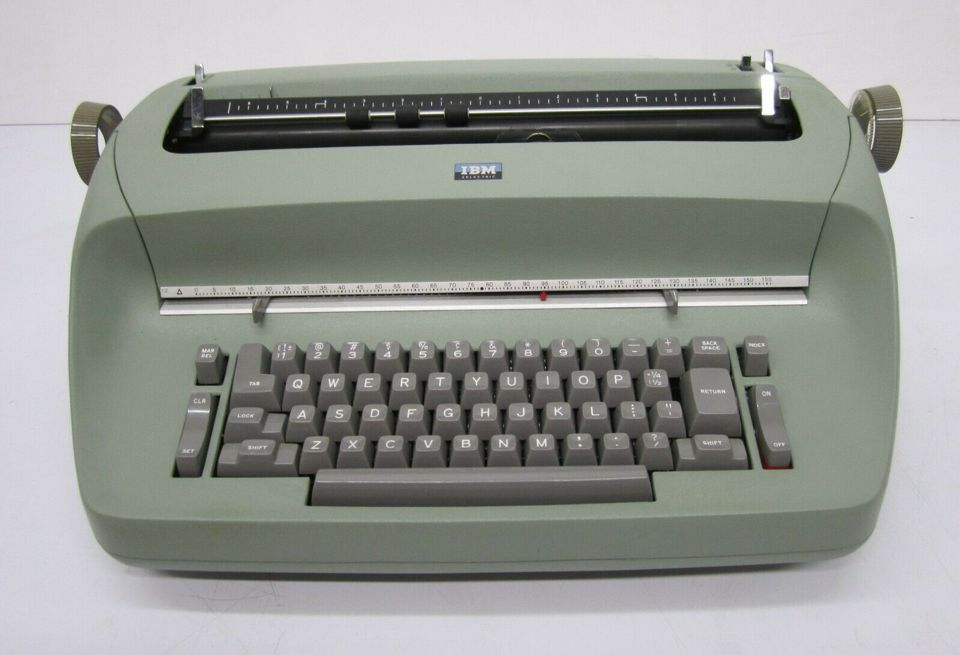
\includegraphics[width=0.46\textwidth]{./Imagenes/Bitmap/selectric.jpg}
     }
     \hfill
     \subfloat[Teclado Bluetooth\label{teclado2}]{%
       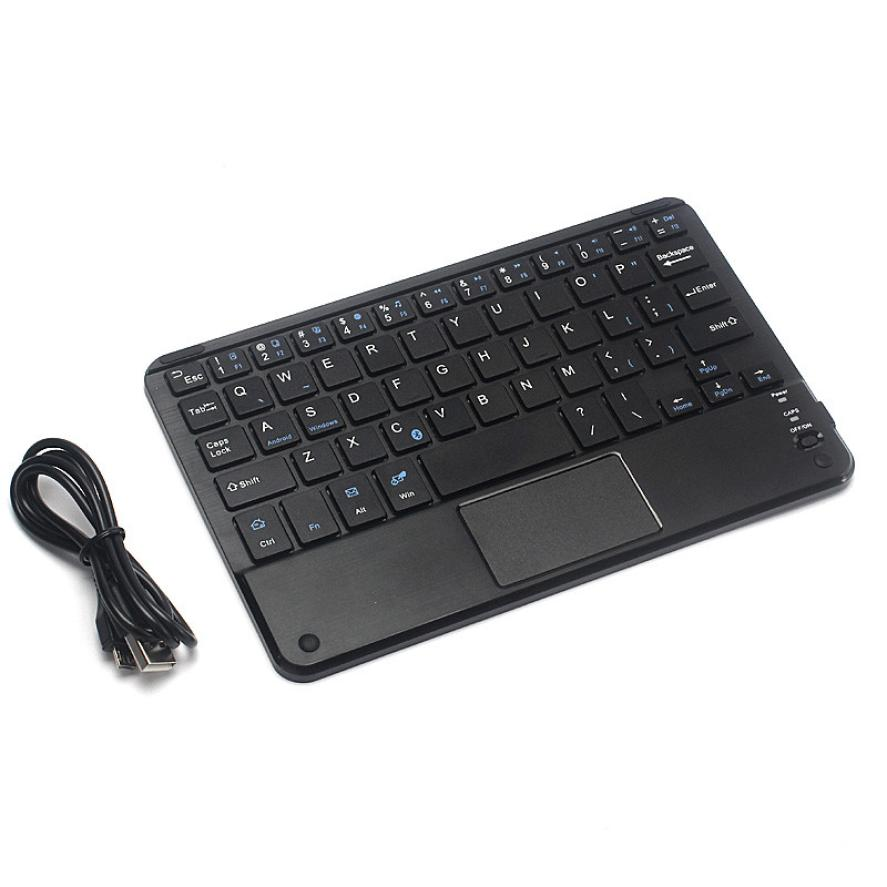
\includegraphics[width=0.46\textwidth]{./Imagenes/Bitmap/teclado-bluetooth.jpg}
     }
     \caption{Evoluci\'on de los teclados}
     \label{fig:primera}
   \end{figure}

%%%%%%%%%%%%%%%%%%%%%%%%%%%%%%%%%%%%%%%%%%%%%%%%%%%%%%%%%%%%%%%%%%
\subsection{Evoluci\'on de los ratones}

Adem\'as del teclado, el segundo dispositivo de entrada por excelencia es el rat\'on. La primera maqueta (figura~\ref{Fig:primerraton}) fue dise\~nada durante los a\~nos 60, dispon\'ia de 2 ruedas met\'alicas que al desplazarse por una superficie mov\'ian 2 ejes. Cada uno de estos ejes controlaba el movimiento tanto vertical como horizontal del cursor en la pantalla y dispon\'ia de un bot\'on en la parte superior con el que se permit\'ia hacer clic en la posici\'on en la que se encontraba el cursor.\\

\begin{figure}[t]
\centering
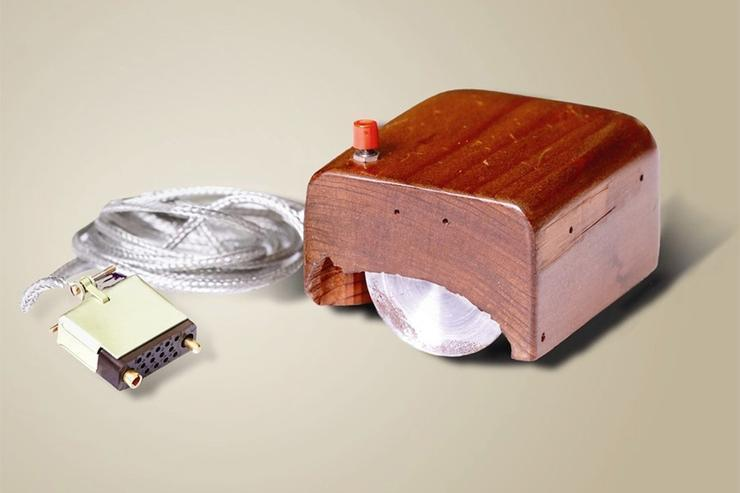
\includegraphics[width=0.29\textwidth]{./Imagenes/Bitmap/Primer_raton.jpg}
\caption{Primer rat\'on desarrollado por Douglas Engelbart y Bill English}
\label{Fig:primerraton}
\end{figure}

El siguiente avance del dispositivo fue cambiar su carcasa de madera por una de pl\'astico y a\~nadir m\'as botones. Tal y como describi\'o \cite{xerox} en su art\'iculo, este avance suele ser atribuido a Microsoft o a Apple. Lejos de ser as\'i, fue la empresa \textbf{Xerox} la que realiz\'o el nuevo dise\~no del rat\'on (figura~\ref{Fig:xerox}) y del que es considerado el primer ordenador personal de la historia junto al Altair 8080. Este nuevo dispositivo sustitu\'ia las 2 ruedas que marcaban la posici\'on del cursor por una \'unica bola de metal. La posici\'on relativa de esta bola era la que determinaba la posici\'on del cursor en la pantalla. \\

\begin{figure}[t]
\begin{minipage}{0.9\textwidth}
    \centering
    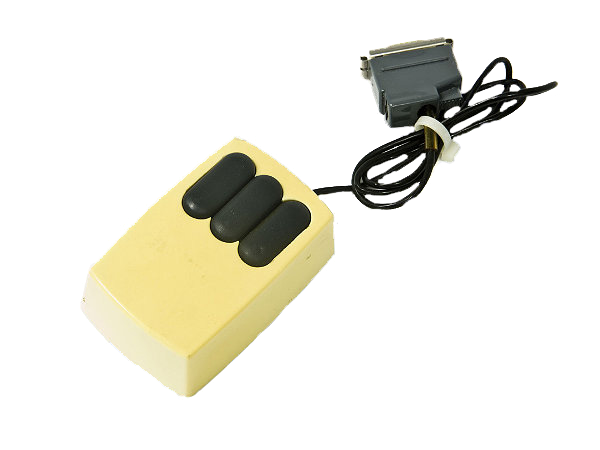
\includegraphics[width=0.40\textwidth]{./Imagenes/Bitmap/mouse_xerox_alto(1).png}
    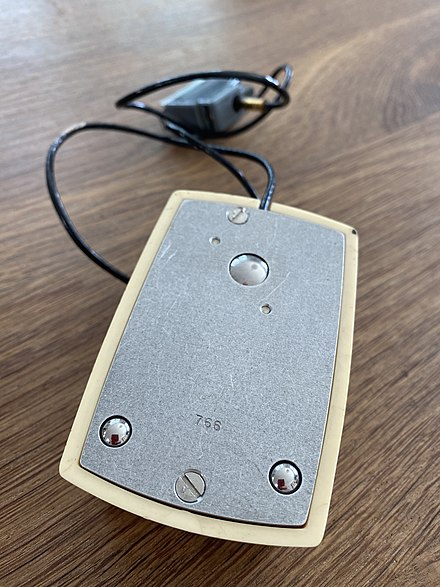
\includegraphics[width=0.20\textwidth]{./Imagenes/Bitmap/mouse_xerox_alto(2).jpg}
\end{minipage}
    \caption{Rat\'on del Xerox Alto de los a\~nos 70}
\label{Fig:xerox}
\end{figure}

En el a\~no 1992 Microsoft decidi\'o vender en un mismo paquete su \'ultima versi\'on de MS-DOS y Windows 3.1, lo que hizo que el rat\'on pasase a ser un perif\'erico fundamental. Se dejaba atr\'as el mundo del texto y se abr\'ian a todos los p\'ublicos las interfaces gr\'aficas del PC. Este cambio hizo que el rat\'on siguiera evolucionando y durante la d\'ecada de los 90 e inicios del 2000 los ratones sufrieron algunas mejoras. Algunas de estas mejoras son: una rueda central o lateral para el desplazamiento, el sensor de movimiento \'optico por diodo led o un sensor basado en un l\'aser no visible. Un sector que aprovech\'o mucho esta estandarizaci\'on del rat\'on y de las interfaces gr\'aficas fue el de los videojuegos. El rat\'on se ha convertido en una parte esencial del mundo de los videojuegos de PC, sirviendo no solo para seleccionar y accionar objetos en pantalla en juegos de estrategia, sino para controlar la c\'amara o cambiar la direcci\'on del personaje en juegos de primera y tercera persona.\\


%%%%%%%%%%%%%%%%%%%%%%%%%%%%%%%%%%%%%%%%%%%%%%%%%%%%%%%%%%%%%%%%%%
\section{Evoluci\'on de los gamepads a trav\'es de las generaciones de consolas}

Se dice que el primer intento de videojuego es una patente de 1947 sobre la simulaci\'on del lanzamiento de misiles pero no fue hasta 1958 y la salida del famoso \textbf{Tenis para Dos} creado por William Higginbotham que se puede comenzar a hablar de videojuegos \citep{tenispara2}. En este juego se recreaba una pista de tenis en la que la pelota iba de un lado a otro de la pista. Poco despu\'es, en 1962 vio la luz \textbf{Spacewar!}. Este t\'itulo fue desarrollado por Steve Russell y posteriormente modificado por sus estudiantes. En este juego lo que se quer\'ia era simular una pelea entre 2 naves en el espacio, fue el primer paso de los juegos multijugador en un mismo dispositivo. El dispositivo de entrada de este juego consist\'ia en 2 ejes de rotaci\'on que se usaban para controlar la rotaci\'on y el empuje de la nave. Adem\'as de esto, el mando dispon\'ia de un bot\'on para disparar misiles (figura~\ref{Fig:spacewar}).\\


\begin{figure}[t]
\centering
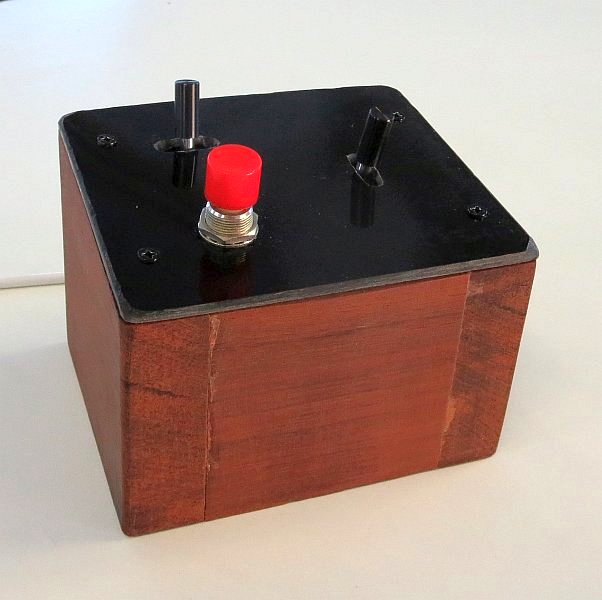
\includegraphics[width=0.4\textwidth]{./Imagenes/Bitmap/spacewar-controller.jpg}
\caption{Joystick utilizado para jugar a Spacewar!}
\label{Fig:spacewar}
\end{figure}

Ser\'a en la d\'ecada de los 70 cuando las m\'aquinas recreativas comiencen a tener repercusi\'on con la salida de \textbf{Pong} en 1972 y \textbf{Space Invaders} en 1978. Muchos t\'itulos y sagas tienen su inicio en esta \'epoca en la que las salas de recreativas estaban abarrotadas de j\'ovenes dispuestos a pasar all\'i todas las horas posibles jugando y compitiendo con otros jugadores. La salida de las consolas, las r\'apidas mejoras del hardware y el avance la tecnolog\'ia hizo que las m\'aquinas recreativas se quedasen obsoletas en poco tiempo. Adem\'as de esto la proliferaci\'on de los cibercaf\'es y los juegos en linea hicieron que el consumo de m\'aquinas arcade se estancara. \\

%%%%%%%%%%%%%%%%%%%%%%%%%%%%%%%%%%%%%%%%%%%%%%%%%%%%%%%%%%%%%%%%%%
\subsection{Primera generaci\'on (1972-1976)}


En 1972 fue lanzada de manera oficial la \textbf{Magnavox Odyssey} y fue considerada la primera videoconsola. El dispositivo de entrada para poder jugar consit\'ia de 2 diales que se utilizaban para el movimiento horizontal y vertical del personaje como puede verse en la figura~\ref{primera1}. Poco despu\'es de la salida de la consola la misma Magnavox sac\'o su juego de disparos conocido como \textit{Magnavox Odyssey Shooting Gallery} en 1972. Este juego ten\'ia la particularidad de que ten\'ia que ser jugado con un mando diferente al original de la consola. Este accesorio nuevo era una pistola de luz (figura~\ref{primera2}). El funcionamiento de este nuevo mando era que los disparos se registraban siempre y cuando la pistola apuntase a una luz intensa por lo que si el jugador apuntaba hacia una bombilla, el juego marcaba como ``alcanzado'' el primer objetivo de la pantalla. La primera soluci\'on de este problema fue dibujar la pantalla en negro una vez el objetivo es alcanzado para asi comprobar que se est\'a apuntando a la pantalla. \\

\begin{figure}[t]
     \subfloat[Magnavox Odyssey joystick\label{primera1}]{%
       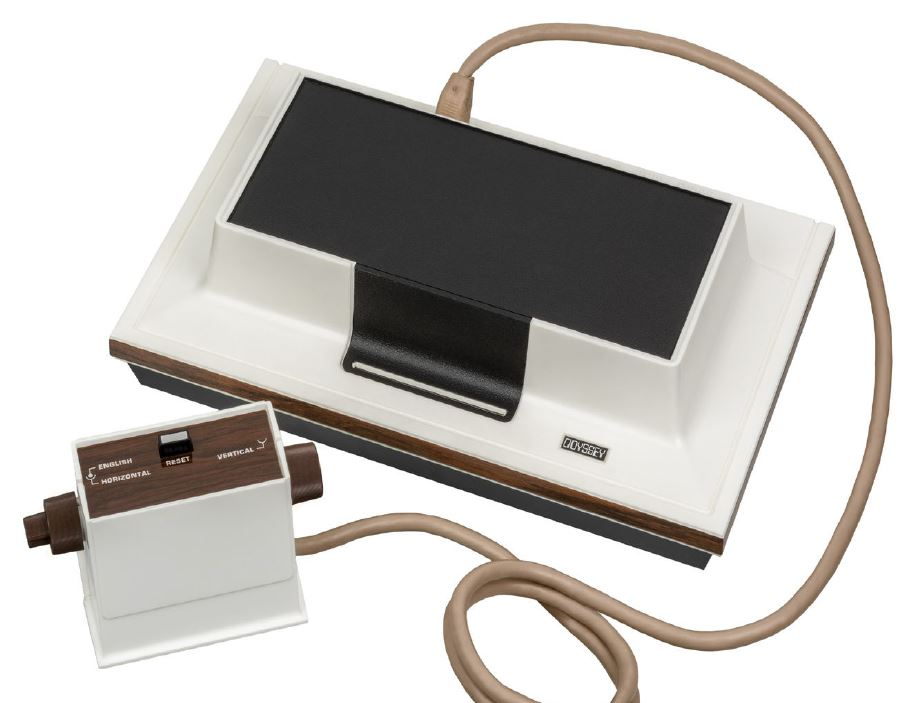
\includegraphics[width=0.4\textwidth]{./Imagenes/Bitmap/Magnavox-Odyssey-Controller.jpg}
     }
     \hfill
     \subfloat[Rifle de luz Magnavox Odyssey Shooting Gallery\label{primera2}]{%
       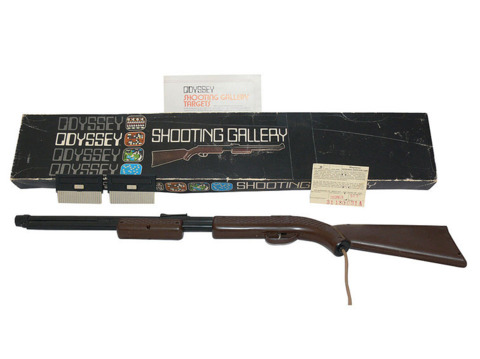
\includegraphics[width=0.4\textwidth]{./Imagenes/Bitmap/pistolaluz.jpg}
     }
     \caption{Dispositivos de entrada relevantes en la 1"a  generaci\'on de consolas}
     \label{fig:primera}
   \end{figure}

%%%%%%%%%%%%%%%%%%%%%%%%%%%%%%%%%%%%%%%%%%%%%%%%%%%%%%%%%%%%%%%%%%
\subsection{Segunda generaci\'on (1976-1983)}


En 1976 la empresa Fairchild Semiconductor sac\'o al mercado la \textbf{Fairchild Channel F} cuya caracter\'istica principal a nivel de entrada de usuario fue la incorporaci\'on de un joystick de 8 direcciones.  Adem\'as de ofrecer un movimiento en 8 direcciones, la parte de arriba de este mando pod\'ia girarse para ser compatible con juegos como \textit{Pong} y tambi\'en pod\'ia ser pulsado y usarse normalmente como bot\'on de disparo, tal y como puede verse en la figura~\ref{segunda1}. \\

En 1977 sali\'o al mercado uno de los joysticks m\'as famosos. Este joystick es el que se utilizaba en la consola \textbf{Atari VCS} que posteriormente ser\'ia conocida como \textbf{Atari 2600}. Este joystick se conoc\'ia como el \textbf{Atari CX40} y consist\'ia de una palanca que permit\'ia un movimiento en 8 direcciones y un bot\'on (figura~\ref{segunda2}). Junto con este modelo, Atari sac\'o al mercado un tipo de conexi\'on que se convertir\'ia en el est\'andar de facto. Los sistemas posteriores eran compatibles con estos joysticks ya que lo tomaron como referencia. Unos pocos a\~nos despu\'es, en 1982, Atari lanz\'o su nueva consola Atari 5200. El sistema combinaba un dise\~no mec\'anico demasiado complejo con un sistema de circuito flexible interno de muy bajo coste. Este controlador incluy\'o un bot\'on de pausa, una caracter\'istica \'unica en ese momento (figura~\ref{segunda3}).\\


\begin{figure}[t]
     \subfloat[Fairchild Channel F joystick\label{segunda1}]{%
       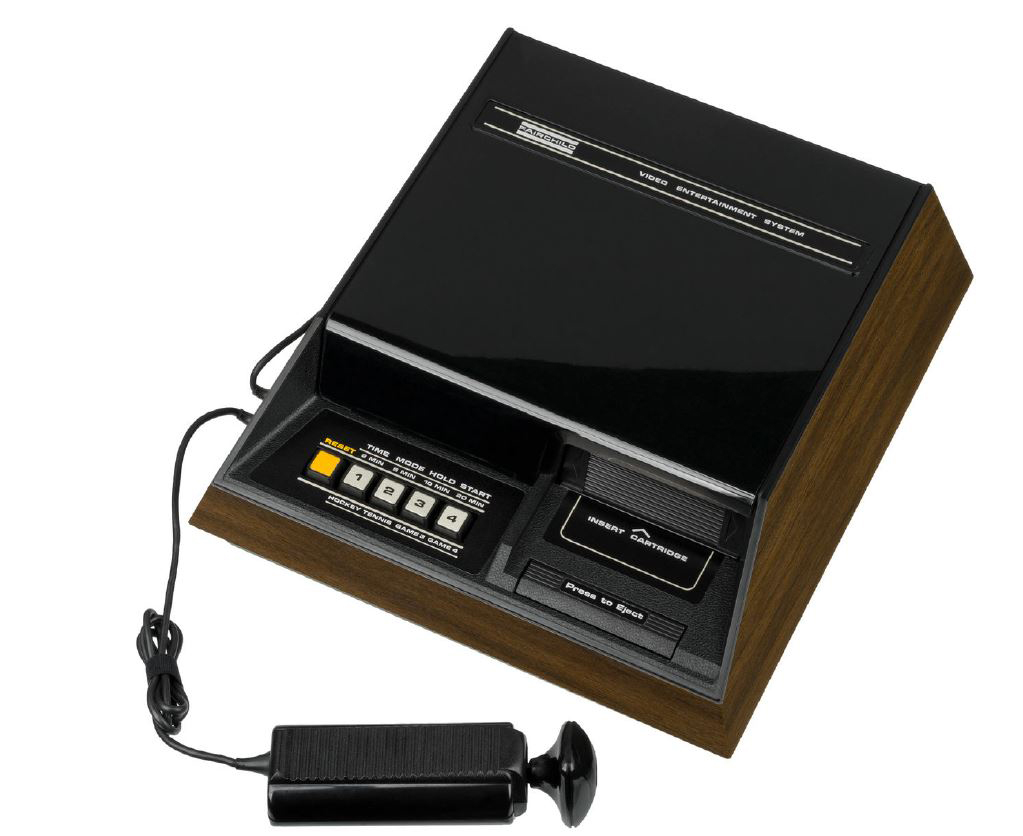
\includegraphics[width=0.3\textwidth]{./Imagenes/Bitmap/Fairchild.jpg}
     }
     \hfill
     \subfloat[AtariCX40\label{segunda2}]{%
       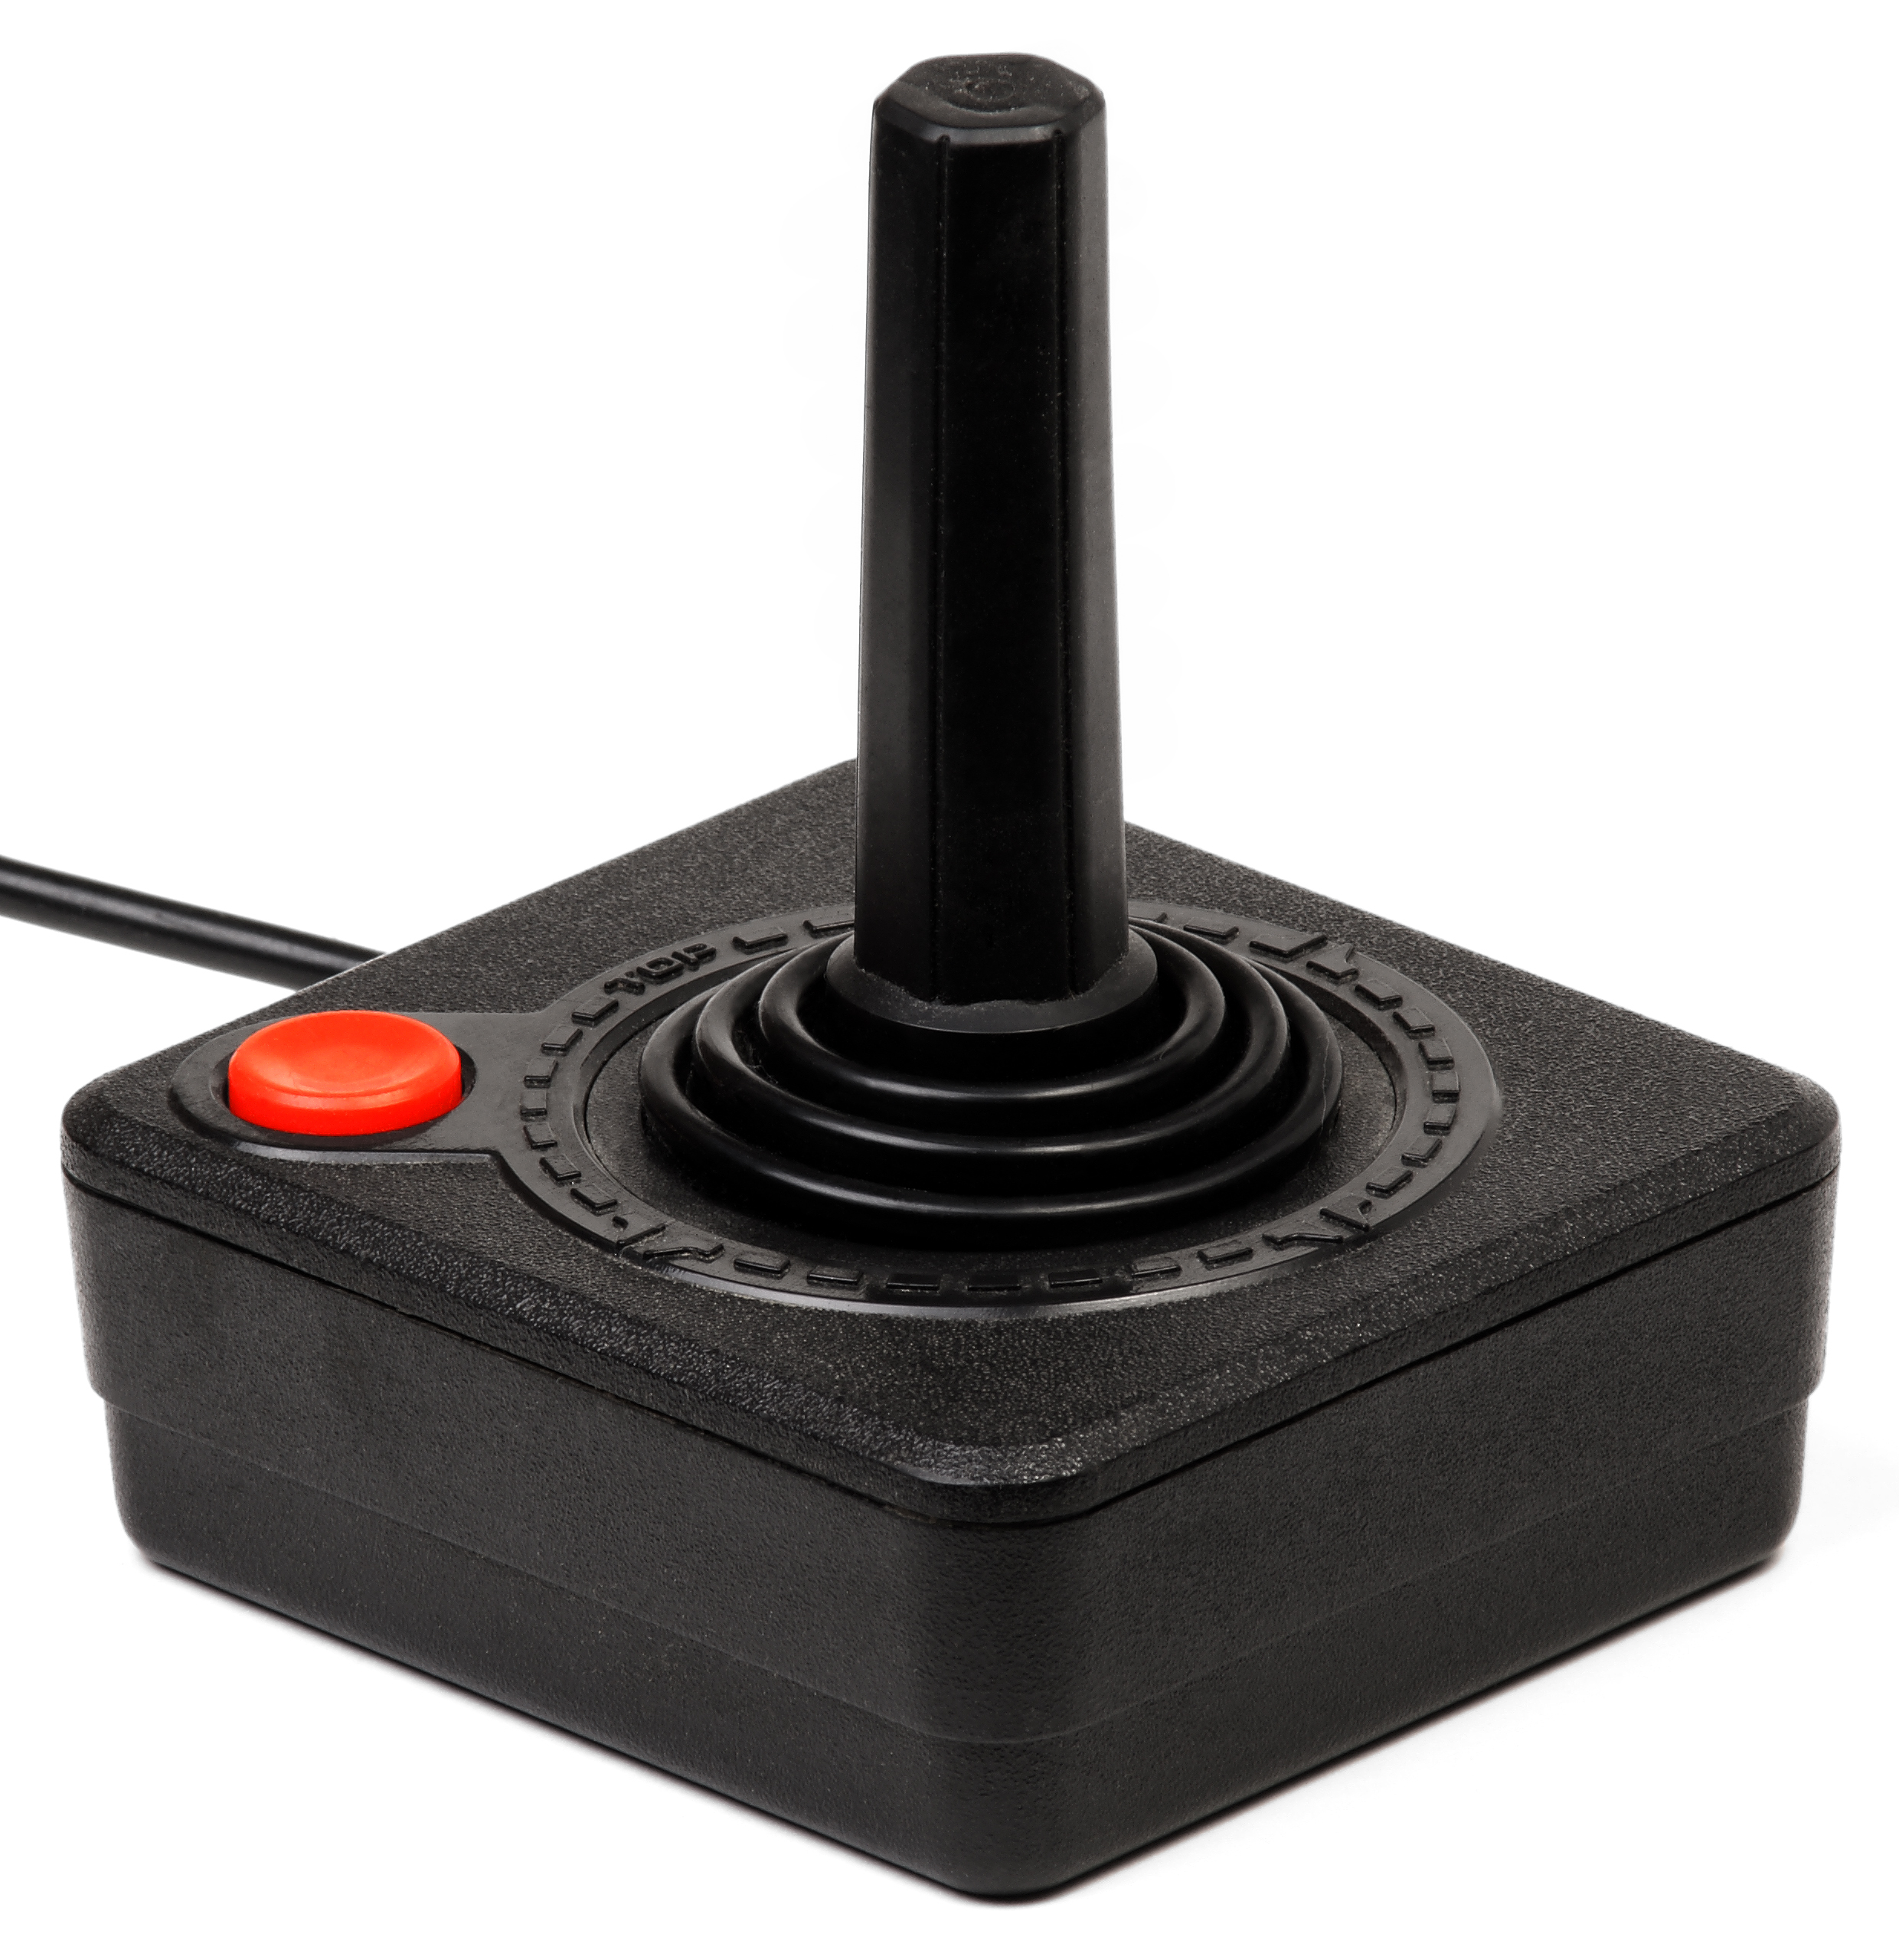
\includegraphics[width=0.3\textwidth]{./Imagenes/Bitmap/Atari-2600-Joystick.jpg}
     }
\hfill
     \subfloat[Atari 5200 joystick\label{segunda3}]{%
       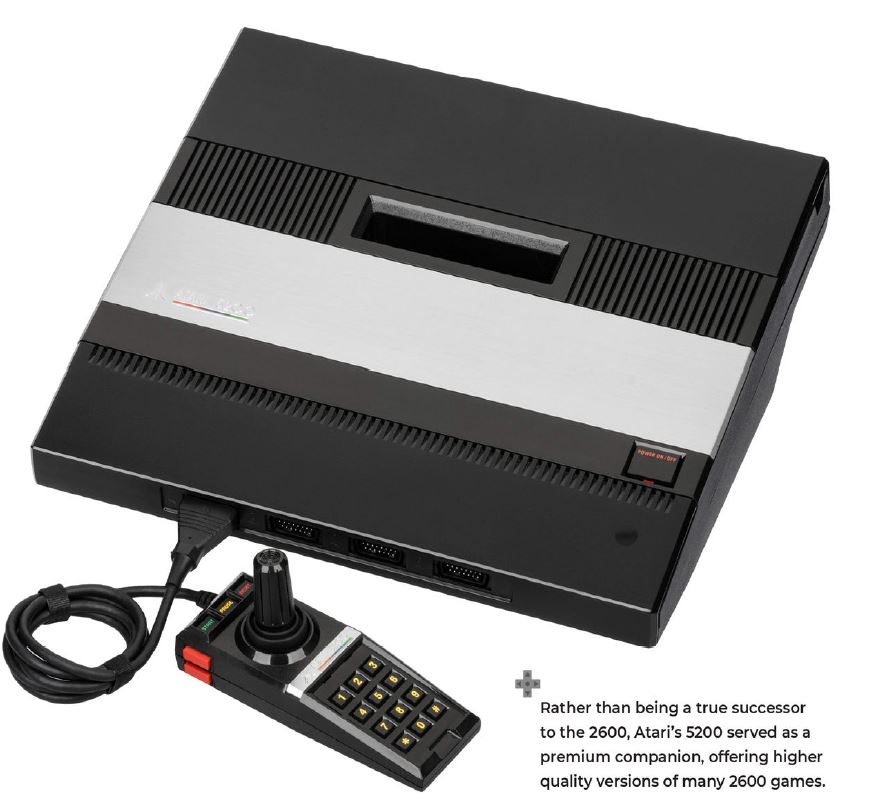
\includegraphics[width=0.3\textwidth]{./Imagenes/Bitmap/1200px-Atari-5200-Controller.png}
     }
     \caption{Dispositivos de entrada relevantes en la 2"a  generaci\'on de consolas}
     \label{fig:segunda}
   \end{figure}

%%%%%%%%%%%%%%%%%%%%%%%%%%%%%%%%%%%%%%%%%%%%%%%%%%%%%%%%%%%%%%%%%%
\subsection{Tercera generaci\'on (1983-1987)}


En 1983 Nintendo sac\'o al mercado \textbf{Nintendo Entertainment System (NES)}. El controlador de esta consola no fue el primer dispositivo donde se utiliz\'o pero el \'exito de la consola lo populariz\'o. Esta cruceta permit\'ia un movimiento en 4 direcciones y que pretend\'ia reemplazar a las voluminosas palancas de mando de los controladores. Adem\'as de la cruceta, el mando dispon\'ia de 2 botones redondos (A y B) y otros 2 botones rectangulares (START y SELECT) tal y como puede verse en la figura~\ref{tercera1}. En lo sucesivo, se lanzaron varios dispositivos especiales dise\~nados precisamente para usarse con juegos espec\'ificos, aunque muy pocos de estos se volvieron populares. Uno de estos dispositivos era el \textbf{Power Glove} (figura~\ref{tercera2}), el que ser\'ia considerado como uno de los primeros perif\'ericos de interfaz en recrear los movimientos de la mano en una pantalla de televisi\'on o de un ordenador en tiempo real. \\

\begin{figure}[t]
     \subfloat[Mando NES\label{tercera1}]{%
       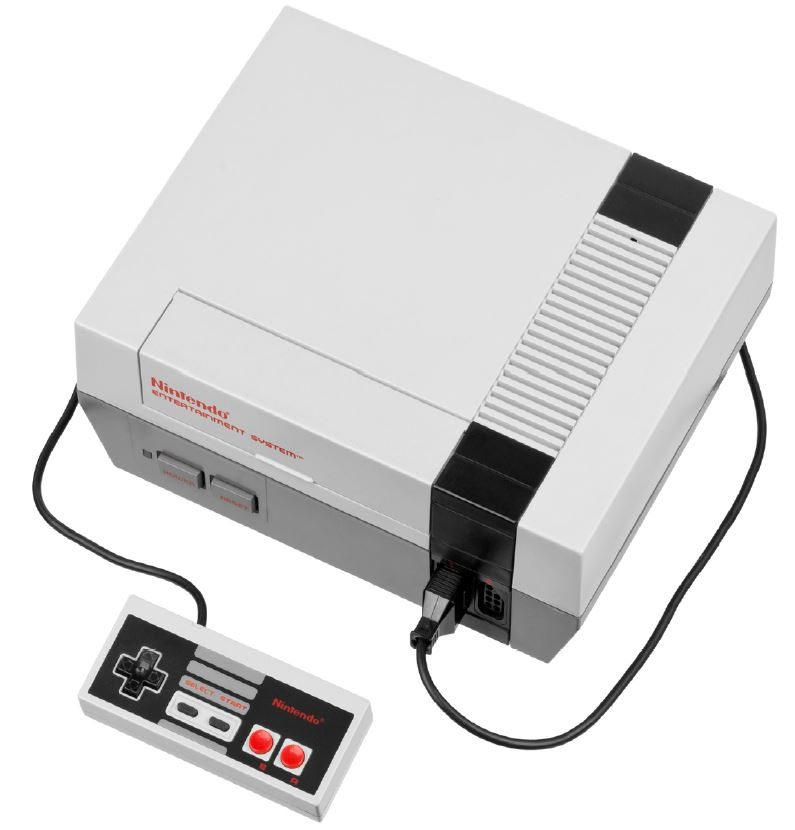
\includegraphics[width=0.5\textwidth]{./Imagenes/Bitmap/NESgamepad.jpg}
     }
     \hfill
     \subfloat[Power Glove NES\label{tercera2}]{%
       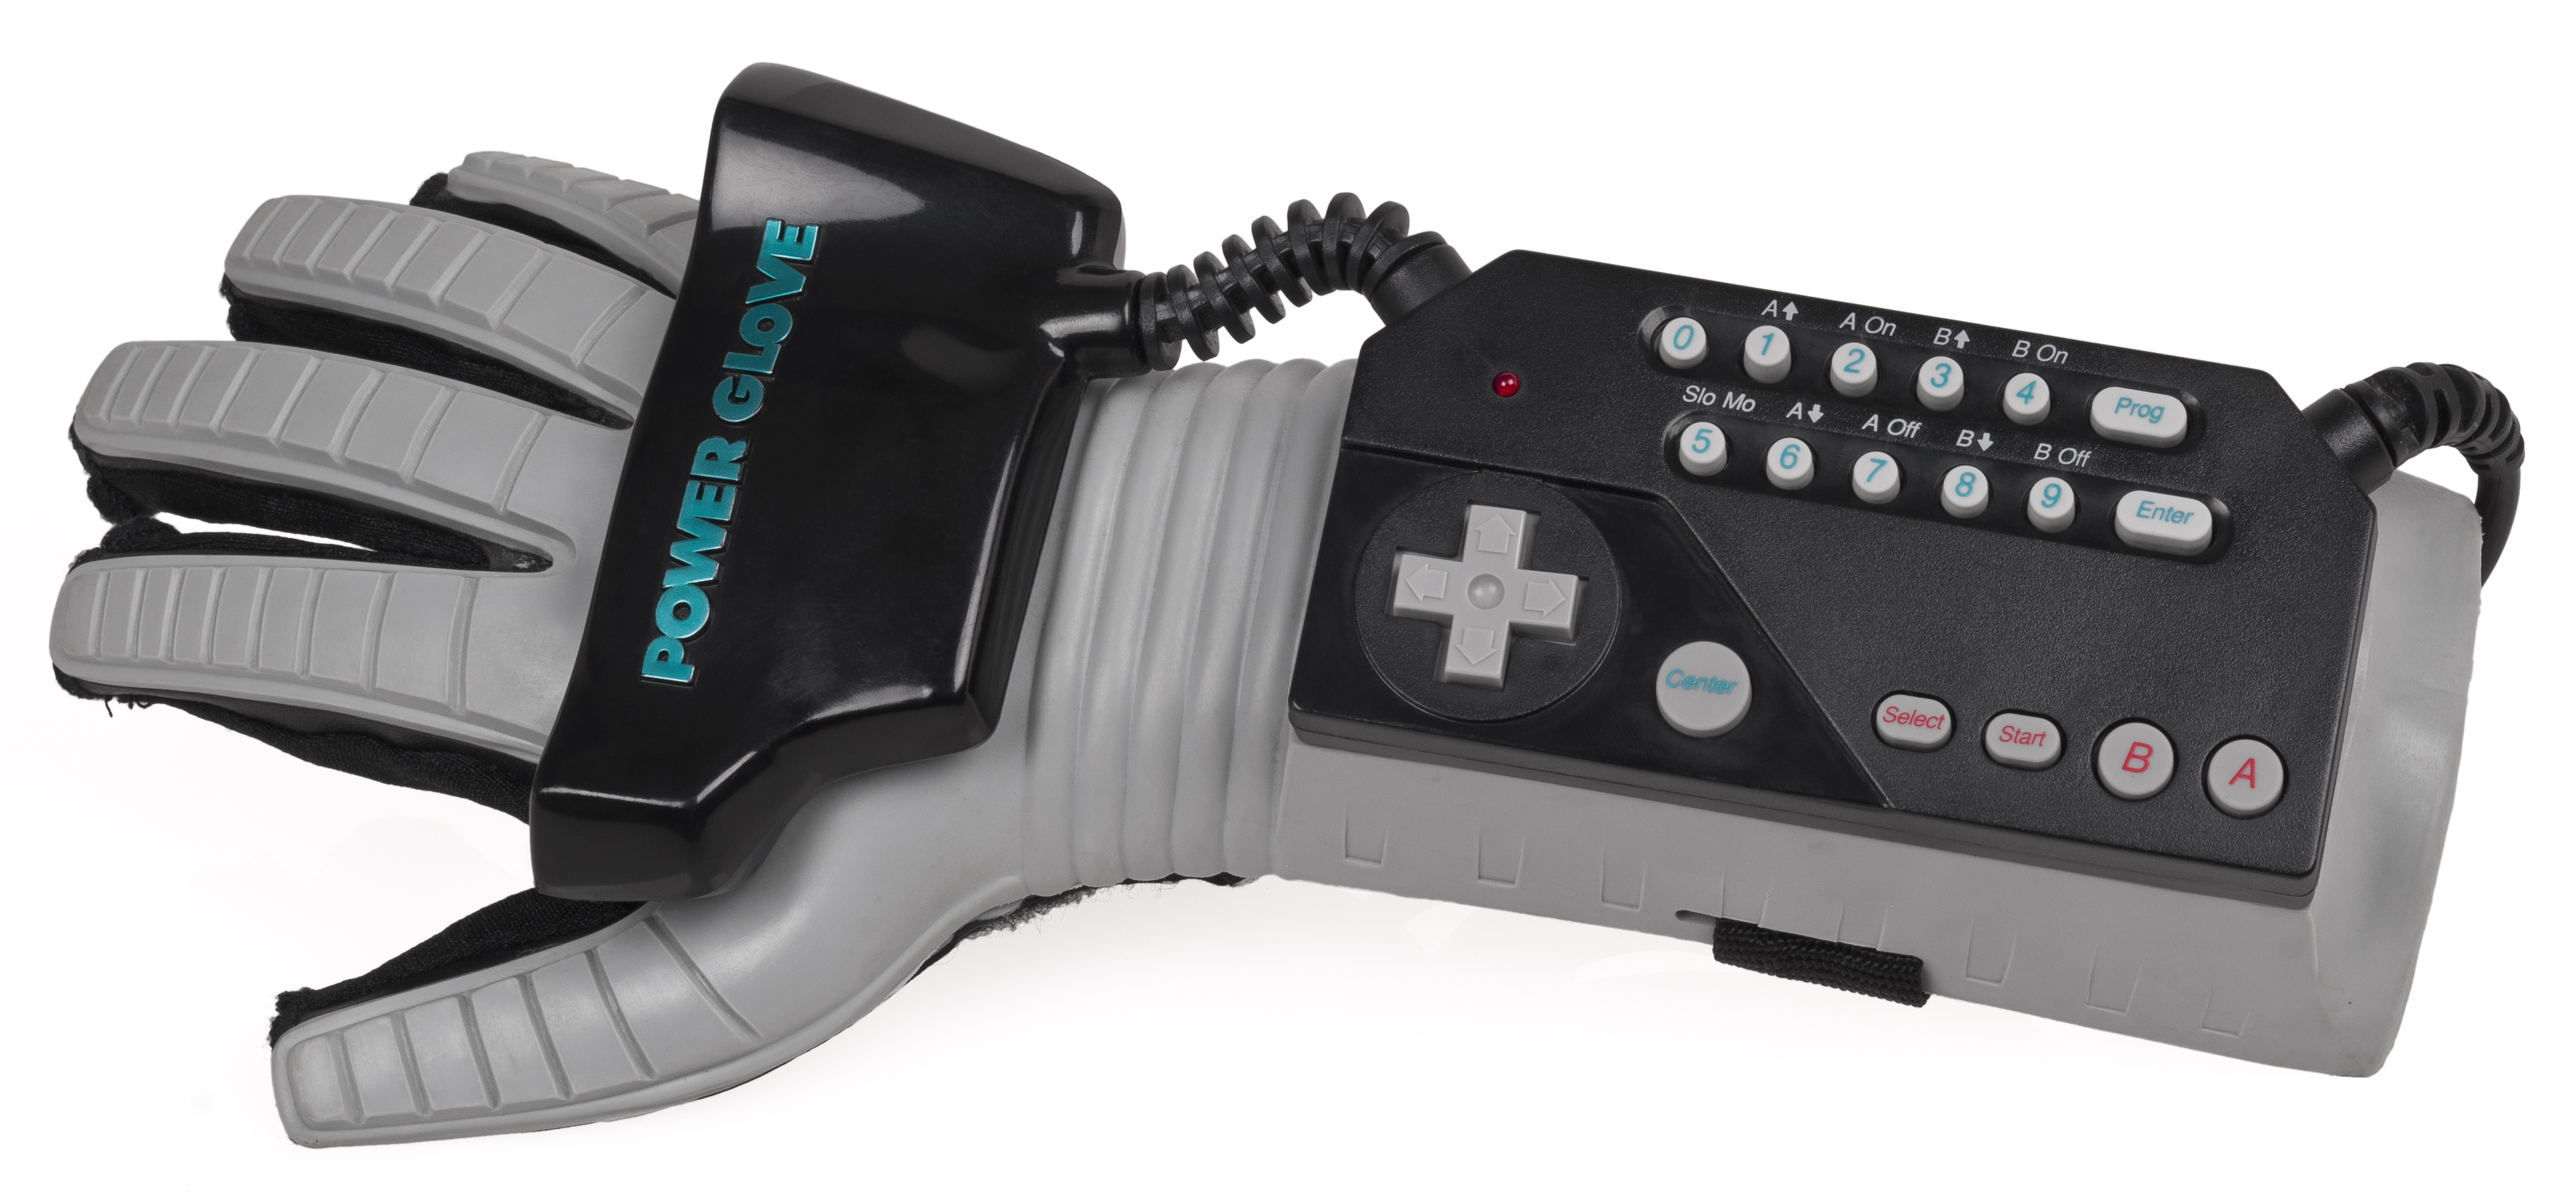
\includegraphics[width=0.5\textwidth]{./Imagenes/Bitmap/NES-Power-Glove.jpg}
     }
     \caption{Dispositivos de entrada relevantes en la 3"a  generaci\'on de consolas}
     \label{fig:tercera}
   \end{figure}

%%%%%%%%%%%%%%%%%%%%%%%%%%%%%%%%%%%%%%%%%%%%%%%%%%%%%%%%%%%%%%%%%%

\subsection{Cuarta generaci\'on (1987-1993)}


En 1990 Nintendo hizo evolucionar a la Nintendo NES y lanz\'o la \textbf{Super Nintendo Entertainment System (SNES)} (figura~\ref{cuarta2}), la cual dej\'o atr\'as un dise\~no cuadrado del controlador y se inclin\'o por un dise\~no m\'as ergon\'omico, se mejor\'o la cruceta y se a\~nadieron otros 2 botones (X e Y). El tiempo de respuesta del controlador era de 16 milisegundos. \\

Dentro de la evoluci\'on de los controladores, en 1993 la compa\~nia SEGA sorprendi\'o con el lanzamiento de un nuevo accesorio para su consola \textbf{Sega Mega Drive}. Este accesorio consist\'ia en un aro octogonal que se colocaba en el suelo y se conectaba directamente al puerto de controlador de la consola. Lo llamaron \textbf{Sega Activator} (figura~\ref{cuarta1}) y fue el primer controladoren el que se utilizaba el cuerpo completo para jugar. El jugador se ten\'ia que situar en el centro del aro, el cual emit\'ia rayos infrarrojos hacia arriba para detectar los movimientos del jugador. Los juegos orientados para el Sega Activator eran juegos que involucrasen el movimiento de brazos y piernas para que el jugador cruzase los rayos infrarrojos y as\'i se detectase el movimiento. Al tratarse de 8 segmentos, cada uno de estos segmentos estaba mapeado como si fuera un bot\'on en el mando tradicional, el cual se ``pulsar\'ia'' cada vez que el jugador cruzase un segmento de los rayos infrarrojos. \\

\begin{figure}[t]
     \subfloat[Sega Activator\label{cuarta1}]{%
       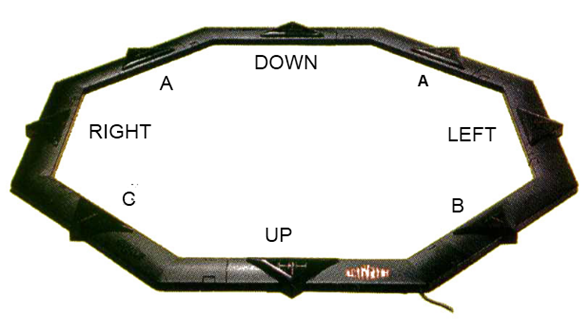
\includegraphics[width=0.45\textwidth]{./Imagenes/Bitmap/SEGAActivator.png}
     }
     \hfill
\subfloat[Super Nintendo joystick\label{cuarta2}]{%
       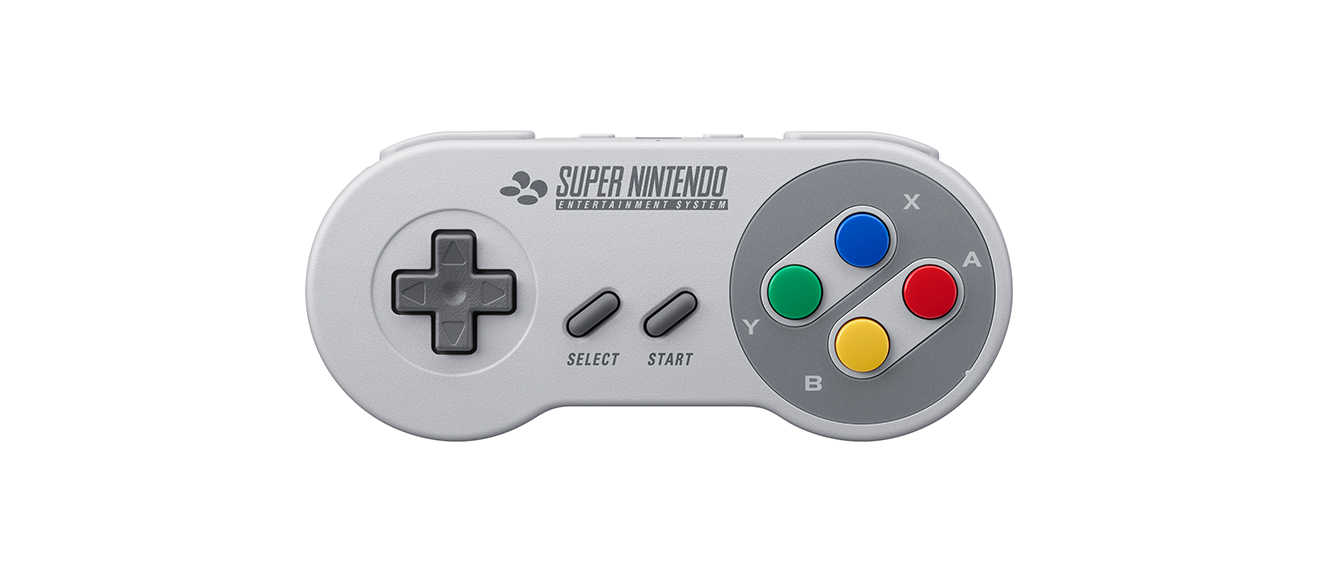
\includegraphics[width=0.5\textwidth]{./Imagenes/Bitmap/SNES.jpg}
     }
     \caption{Dispositivos de entrada relevantes en la 4"a  generaci\'on de consolas}
     \label{fig:cuarta}
   \end{figure}
%%%%%%%%%%%%%%%%%%%%%%%%%%%%%%%%%%%%%%%%%%%%%%%%%%%%%%%%%%%%%%%%%%

\subsection{Quinta generaci\'on (1993-1998)}



Durante los a\~nos 90 \textbf{Sony} entr\'o al terreno del desarrollo de consolas y por consecuencia, de modelos diferentes de controladores de videojuegos. Con su primera consola, la \textbf{Sony PlayStation}, incluyeron un nuevo dise\~no de mando que recog\'ia muchos de los dise\~nos vistos hasta el momento. A diferencia de Nintendo, este controlador cambi\'o la nomenclatura de los botones A, B, Y y X por las figuras $\triangle$, $\textbigcircle$, $\times$ y $\Box$, manten\'ia la cruceta y los botones START y SELECT y adem\'as a\~nadi\'o 4 botones m\'as en la parte lateral del mando para los dedos \'indice y coraz\'on. 3 a\~nos m\'as tarde Sony sacar\'ia una re-edici\'on del mando al que le incorporaron 2 sticks anal\'ogicos junto con un bot\'on con un LED para cambiar entre los diferentes modos usados para el control del personaje (figura~\ref{quinta3}). \'Unicamente la versi\'on japonesa presentaba una funci\'on de retroalimentaci\'on de vibraci\'on. \\

Por el lado de Nintendo, la consola sucesora de la Super Nintendo fue la \textbf{Nintendo 64} que fue acompa\~nada por un nuevo dise\~no de mando que no pas\'o desapercibido (figura~\ref{quinta1}). Dispon\'ia de una cruceta en la parte izquierda del mando, un stick de 360 grados y un bot\'on START en el centro del mando y 6 botones en su parte derecha. Complementario a esto, en la parte trasera del mando hab\'ia 2 botones m\'as y tambi\'en en la parte trasera se daba la opci\'on de introducir un dispositivo extraible que proporcionaba retroalimentaci\'on de vibraci\'on (figura~\ref{quinta2}). Este accesorio se activaba en ocasiones concretas como al disparar un arma y serv\'ia para sumergir al jugador en el videojuego.\\

\begin{figure}[t]
     \subfloat[Mando Nintendo 64\label{quinta1}]{%
       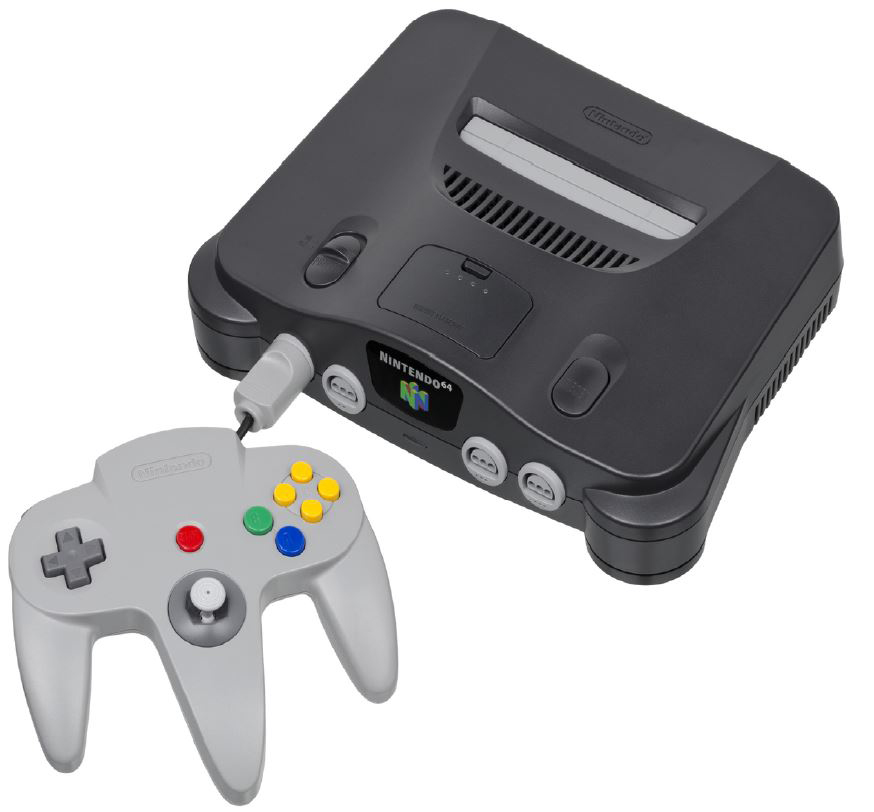
\includegraphics[width=0.3\textwidth]{./Imagenes/Bitmap/N64-Console-Set.png}
     }
     \hfill
 \subfloat[Rumble Pack Nintendo 64\label{quinta2}]{%
       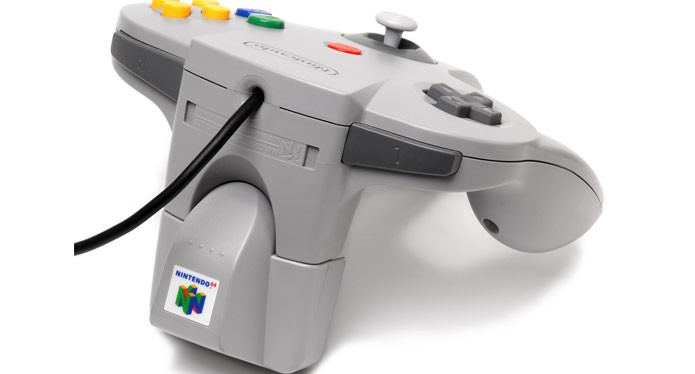
\includegraphics[width=0.3\textwidth]{./Imagenes/Bitmap/rumble-pack-64.jpg}
     }
\hfill
 \subfloat[Dualshock con sticks anal\'ogicos\label{quinta3}]{%
       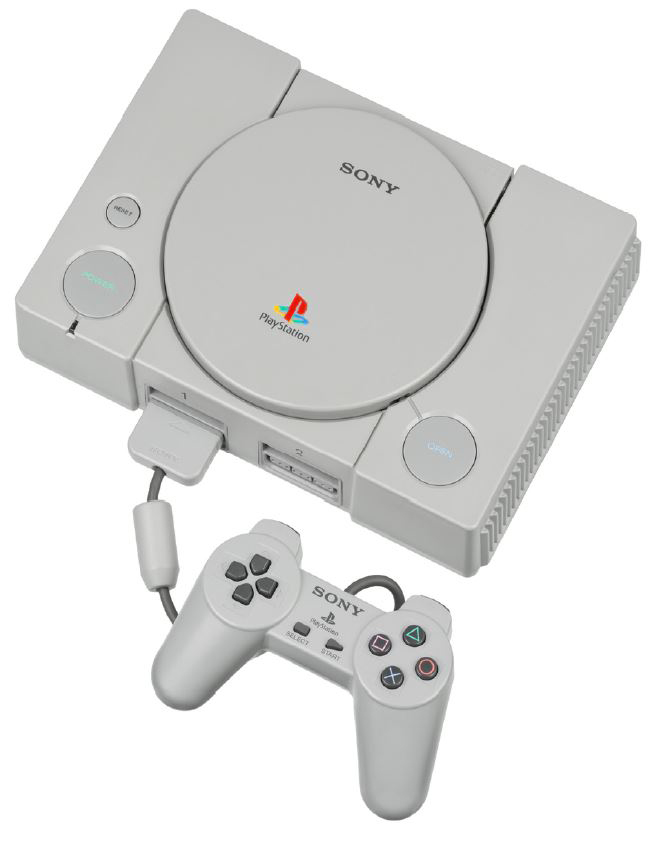
\includegraphics[width=0.3\textwidth]{./Imagenes/Bitmap/Dualshock.jpg}
     }
     \caption{Dispositivos de entrada relevantes en la 5"a  generaci\'on de consolas}
     \label{fig:quinta}
   \end{figure}

%%%%%%%%%%%%%%%%%%%%%%%%%%%%%%%%%%%%%%%%%%%%%%%%%%%%%%%%%%%%%%%%%%

\subsection{Sexta generaci\'on (1998-2005)}

En los a\~nos posteriores las compa\~nias siguieron sacando diferentes mandos que modificaban tama\~no y posiciones de los botones pero no salieron cambios significativos hasta que en 2002 Nintendo lanz\'o al mercado un nuevo mando alternativo para su consola \textbf{GameCube}, este controlador ten\'ia la peculiaridad de ser inal\'ambrico. Lo llamaron \textbf{WaveBird Wireless Controller} (figura~\ref{sexta1}) y sent\'o las bases para los pr\'oximos mandos inal\'ambricos. Contaba con una cruceta, 6 botones digitales, 2 botones h\'ibridos ya que hacian la funci\'on de gatillos y 2 palancas anal\'ogicas para el movimiento del personaje y la c\'amara normalmente. Como alimentaci\'on usaba 2 pilas AA y para comunicarse con la consola usaba radiofrecuencia, lo que permit\'ia al jugador alejarse hasta 6 metros de la consola. Poco tiempo despu\'es tanto Sony con su PlayStation 3 como Microsoft con su Xbox 360 a\~nadir\'ian las baterias a sus mandos para convertirlos en inal\'ambricos. \\


\begin{figure}[t]
     \subfloat[WaveBird Wireless Controller\label{sexta1}]{%
       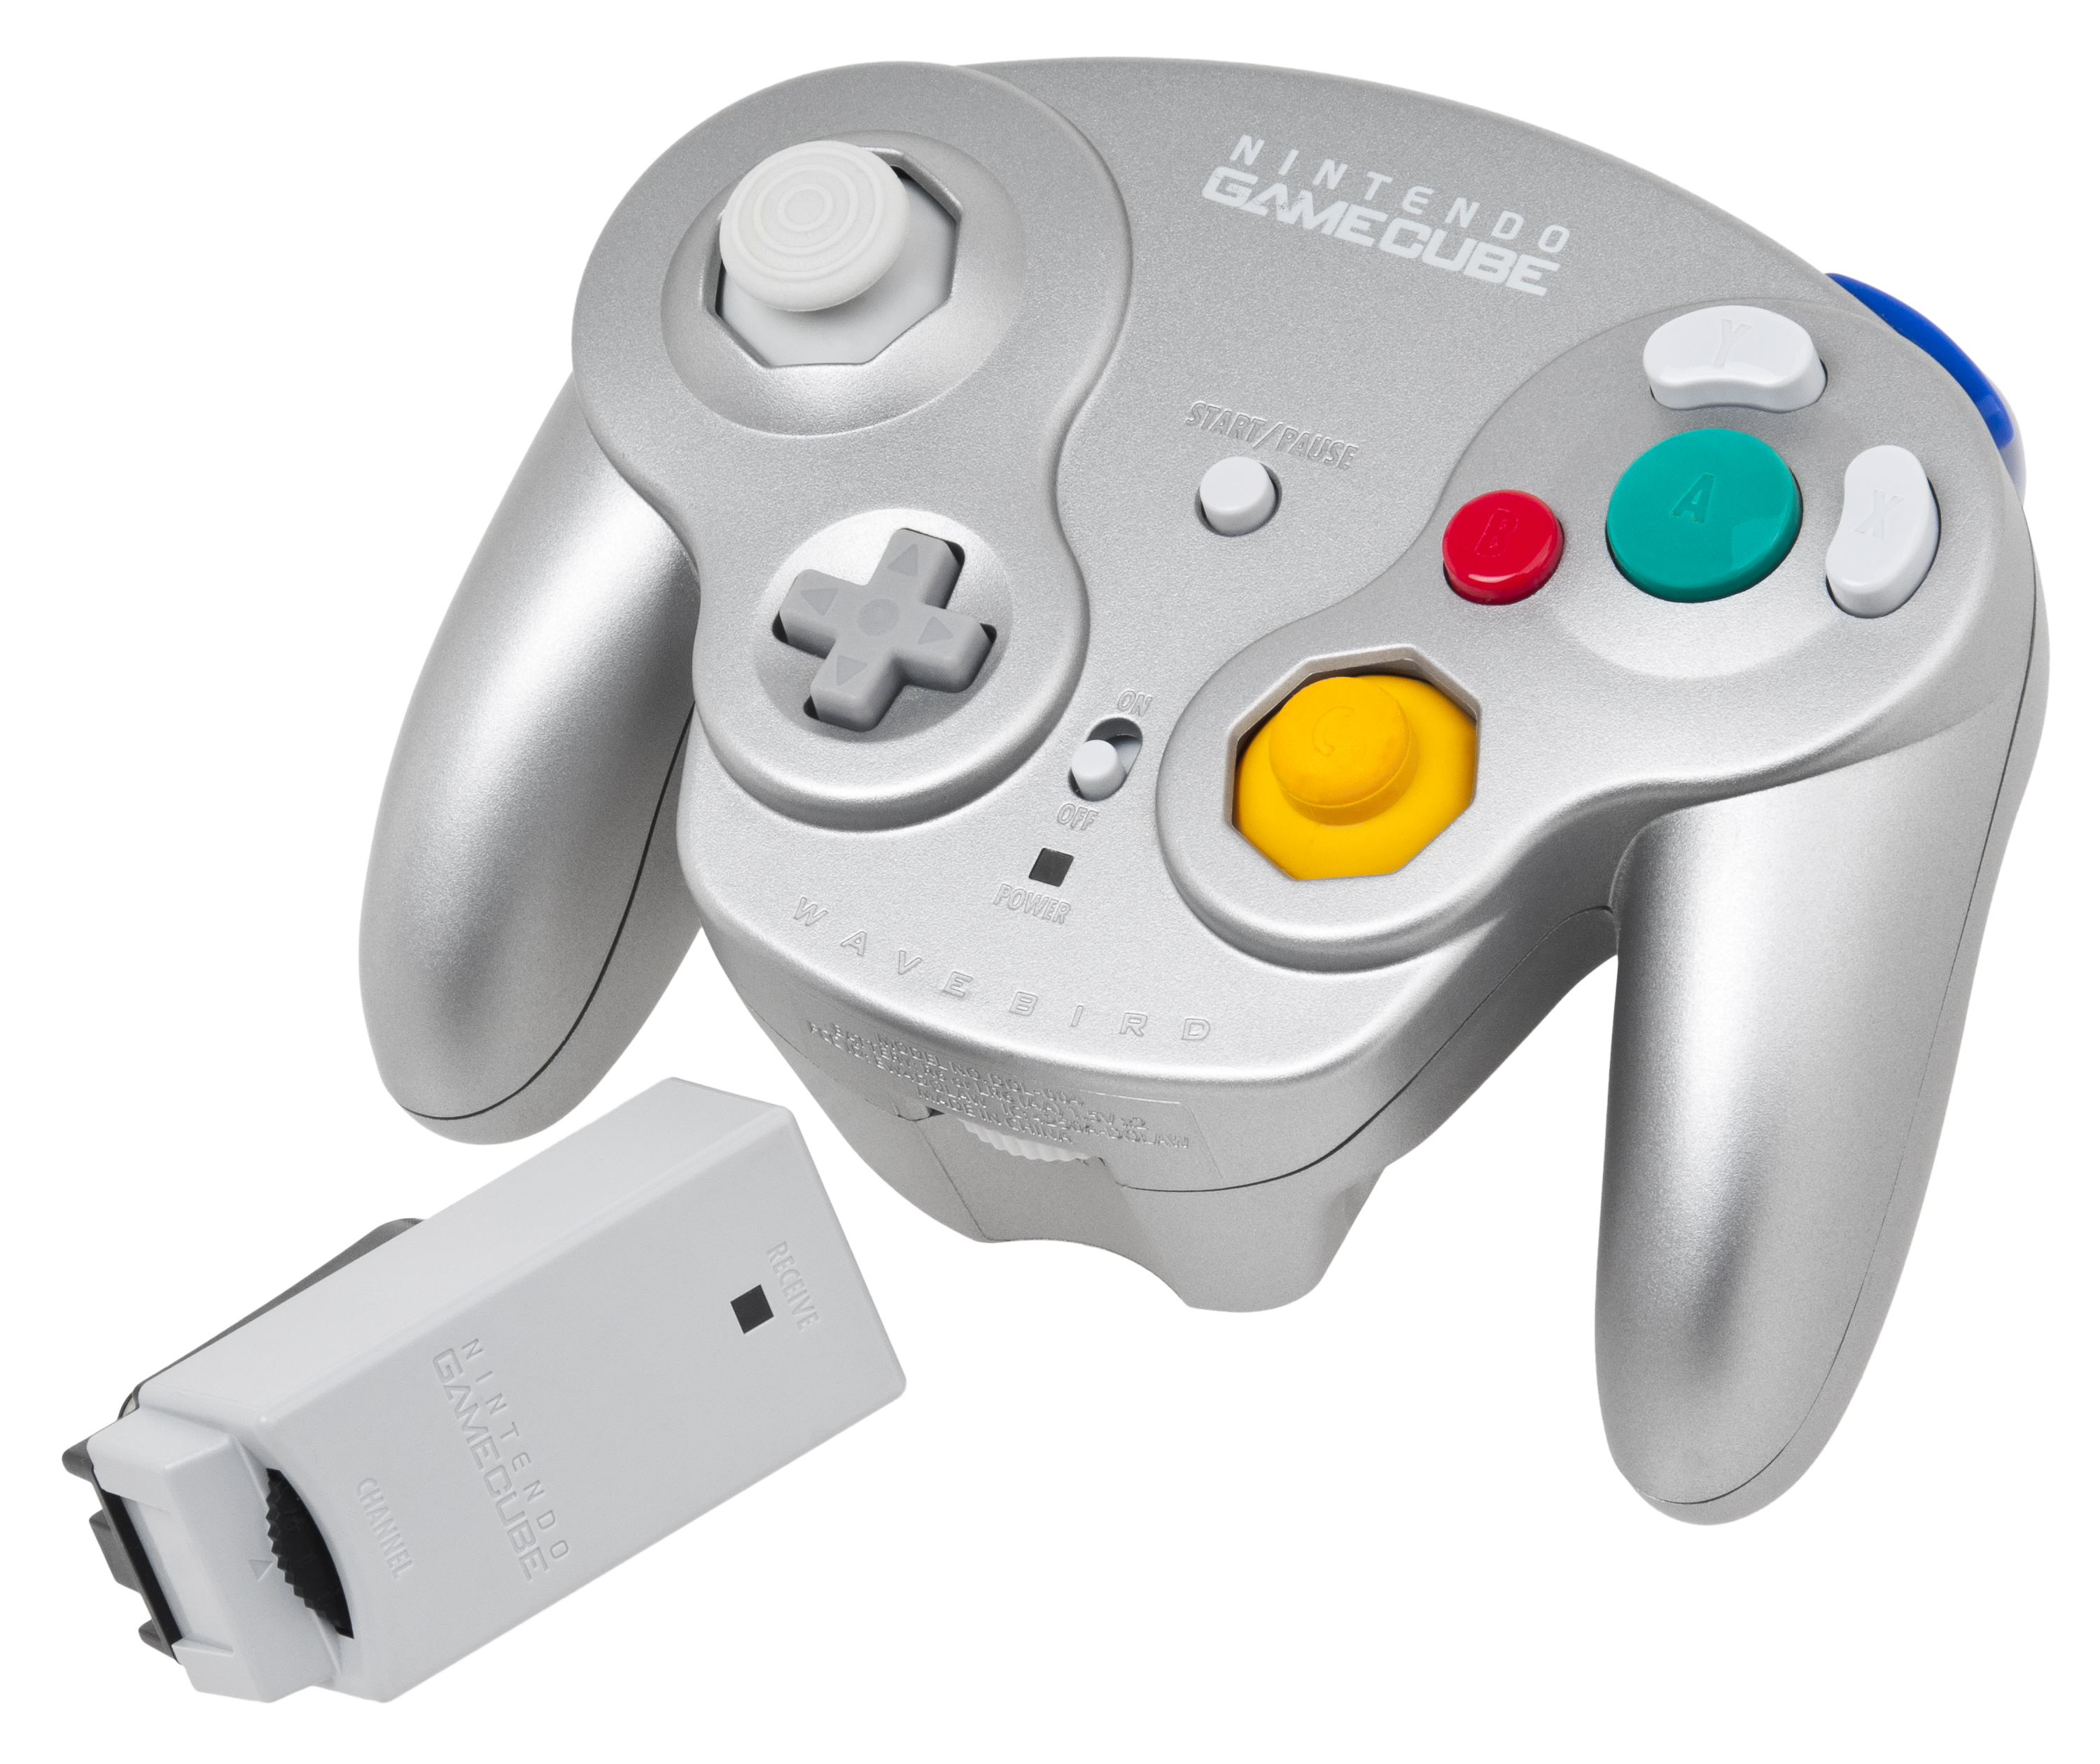
\includegraphics[width=0.4\textwidth]{./Imagenes/Bitmap/Nintendo-GameCube-Wavebird-Silver.jpg}
     }
     \hfill
\subfloat[Joystick original GameCube\label{sexta2}]{%
       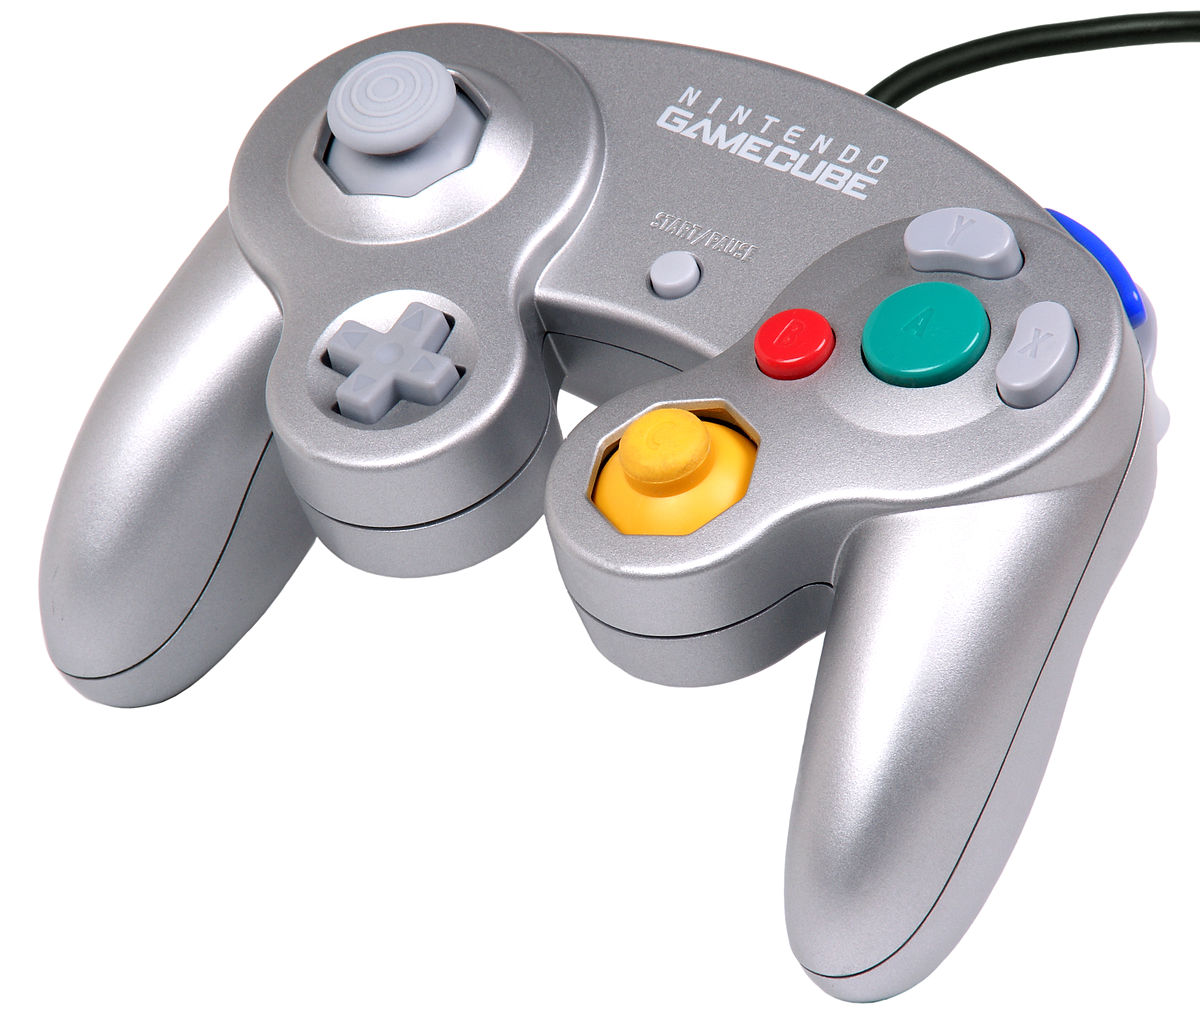
\includegraphics[width=0.4\textwidth]{./Imagenes/Bitmap/1200px-Gamecube-controller.jpg}
     }
     \caption{Dispositivos de entrada relevantes en la 6"a  generaci\'on de consolas}
     \label{fig:sexta}
   \end{figure}

%%%%%%%%%%%%%%%%%%%%%%%%%%%%%%%%%%%%%%%%%%%%%%%%%%%%%%%%%%%%%%%%%%

\subsection{Septa generaci\'on (2005-2012)}

\begin{figure}[t]
     \subfloat[Barra de sensores infrarrojos Wii\label{septa1}]{%
       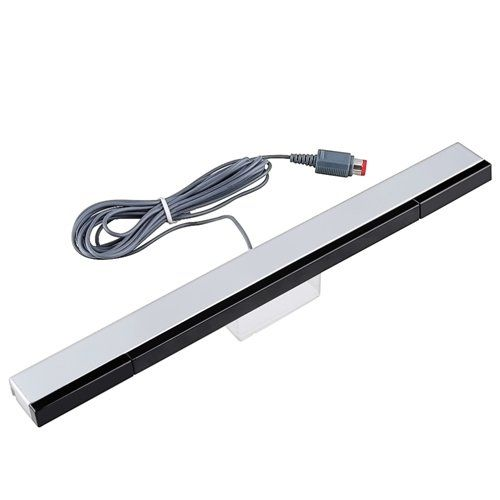
\includegraphics[width=0.5\textwidth]{./Imagenes/Bitmap/barra-sensor-infrarrojos-para-nintendo-wii-con-cable_3.jpg}
     }
     \hfill
\subfloat[Wiimote y Nunchuck\label{septa2}]{%
       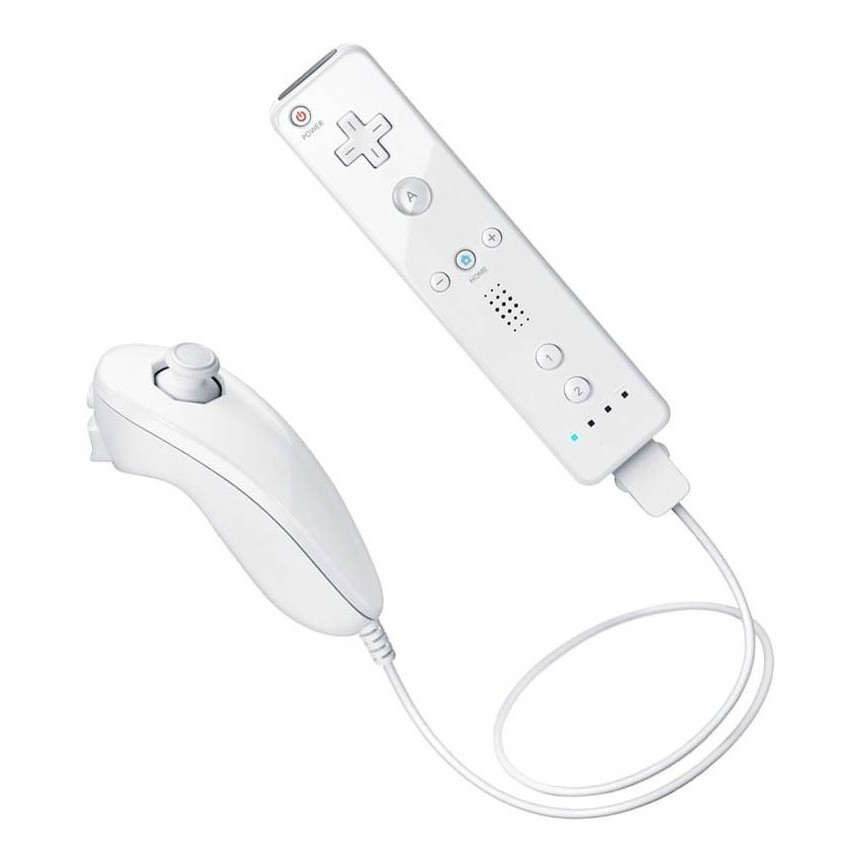
\includegraphics[width=0.5\textwidth]{./Imagenes/Bitmap/wiimote_nunchuck.jpg}
     }
     \caption{Dispositivos de entrada relevantes de Nintendo en la 7"a  generaci\'on}
     \label{fig:septima}
   \end{figure}

En 2006 Nintendo lanz\'o al mercado una consola cuya idea principal era ser usada por todos los miembros de la casa. Esta consola fue \textbf{Wii} y trajo consigo la caracter\'istica m\'as importante de esta consola, una nueva versi\'on de mando. El \textbf{Wiimote} o \textbf{Wii Remote} tiene la capacidad de detectar movimiento en los 3 ejes mediante el uso de aceler\'ometros y la de apuntar. A diferencia de lo que ocurr\'ia con las pistolas de luz, la detecci\'on de la direcci\'on del apuntado ven\'ia dado por una barra de sensores con LED infrarrojos (figura~\ref{septa1}). Para lograr detectar la direcci\'on a la que el Wiimote apunta, el dispositivo incorpora en su parte superior un sensor \'optico \textit{PixArt}. Este dispositivo unido a una barra de 10 sensores LED infrarrojos, permit\'ian al jugador apuntar de manera precisa hasta 5 metros de distancia de la barra. Para que el apuntado fuese m\'as preciso la barra deb\'ia colocarse encima o debajo de la televisi\'on.\\

El dise\~no del controlador es similar a los control remoto de televisi\'on para as\'i hacer que sea lo m\'as intuitivo posible. En su parte frontal, el Wiimote dispone de los botones A, 1, 2, +, -, HOME, POWER y una cruceta. Adem\'as de estos botones el mando incorpora un bot\'on trasero en forma de gatillo y un altavoz en su parte frontal. El mando necesitaba 2 pilas para ser utilizado e inclu\'ia 4 luces numeradas que serv\'ian para ver la carga del mando y el n\'umero del jugador que utilizaba ese mando. El accesorio principal del mando era el \textbf{Nunchuck} que adem\'as ven\'ia incluido con la consola (figura~\ref{septa2}). Nunchuck daba 2 botones adicionales en su parte trasera y un joystick anal\'ogico. Estos accesorios al mando pod\'ian conectarse por un puerto de expansi\'on del que dispon\'ia el mando en la parte inferior. Tambi\'en en la parte inferior ven\'ia incluida una correa con la que poder asegurar el mando a la mu\~neca y evitar que durante una sesi\'on de juego el mando se resbalase de la mano.\\

\begin{figure}[t]
     \subfloat[Kinect\label{septa3}]{%
       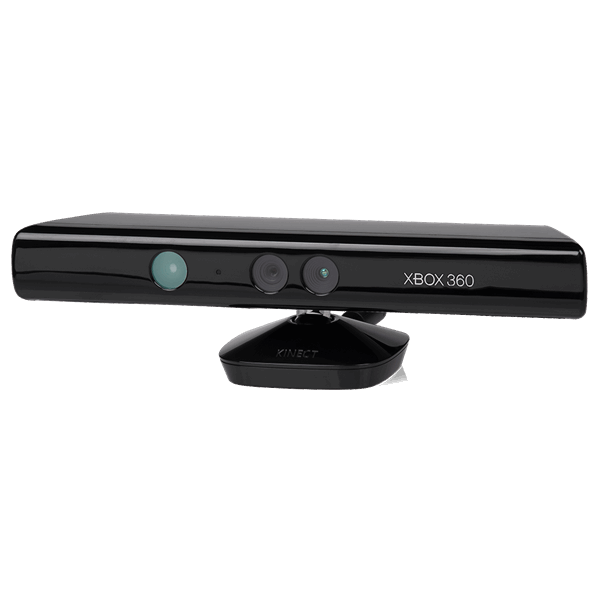
\includegraphics[width=0.3\textwidth]{./Imagenes/Bitmap/Kinect.png}
     }
     \hfill
\subfloat[PlayStation Move con Navigation Controller\label{septa4}]{%
       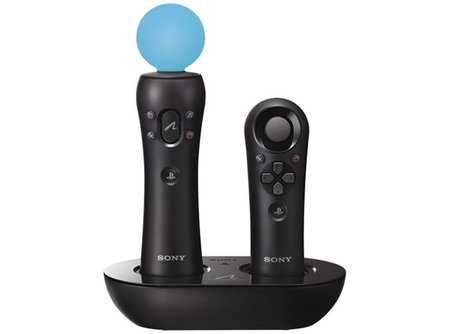
\includegraphics[width=0.3\textwidth]{./Imagenes/Bitmap/PSMove.jpg}
     }
\hfill
\subfloat[PlayStation Eye\label{septa5}]{%
       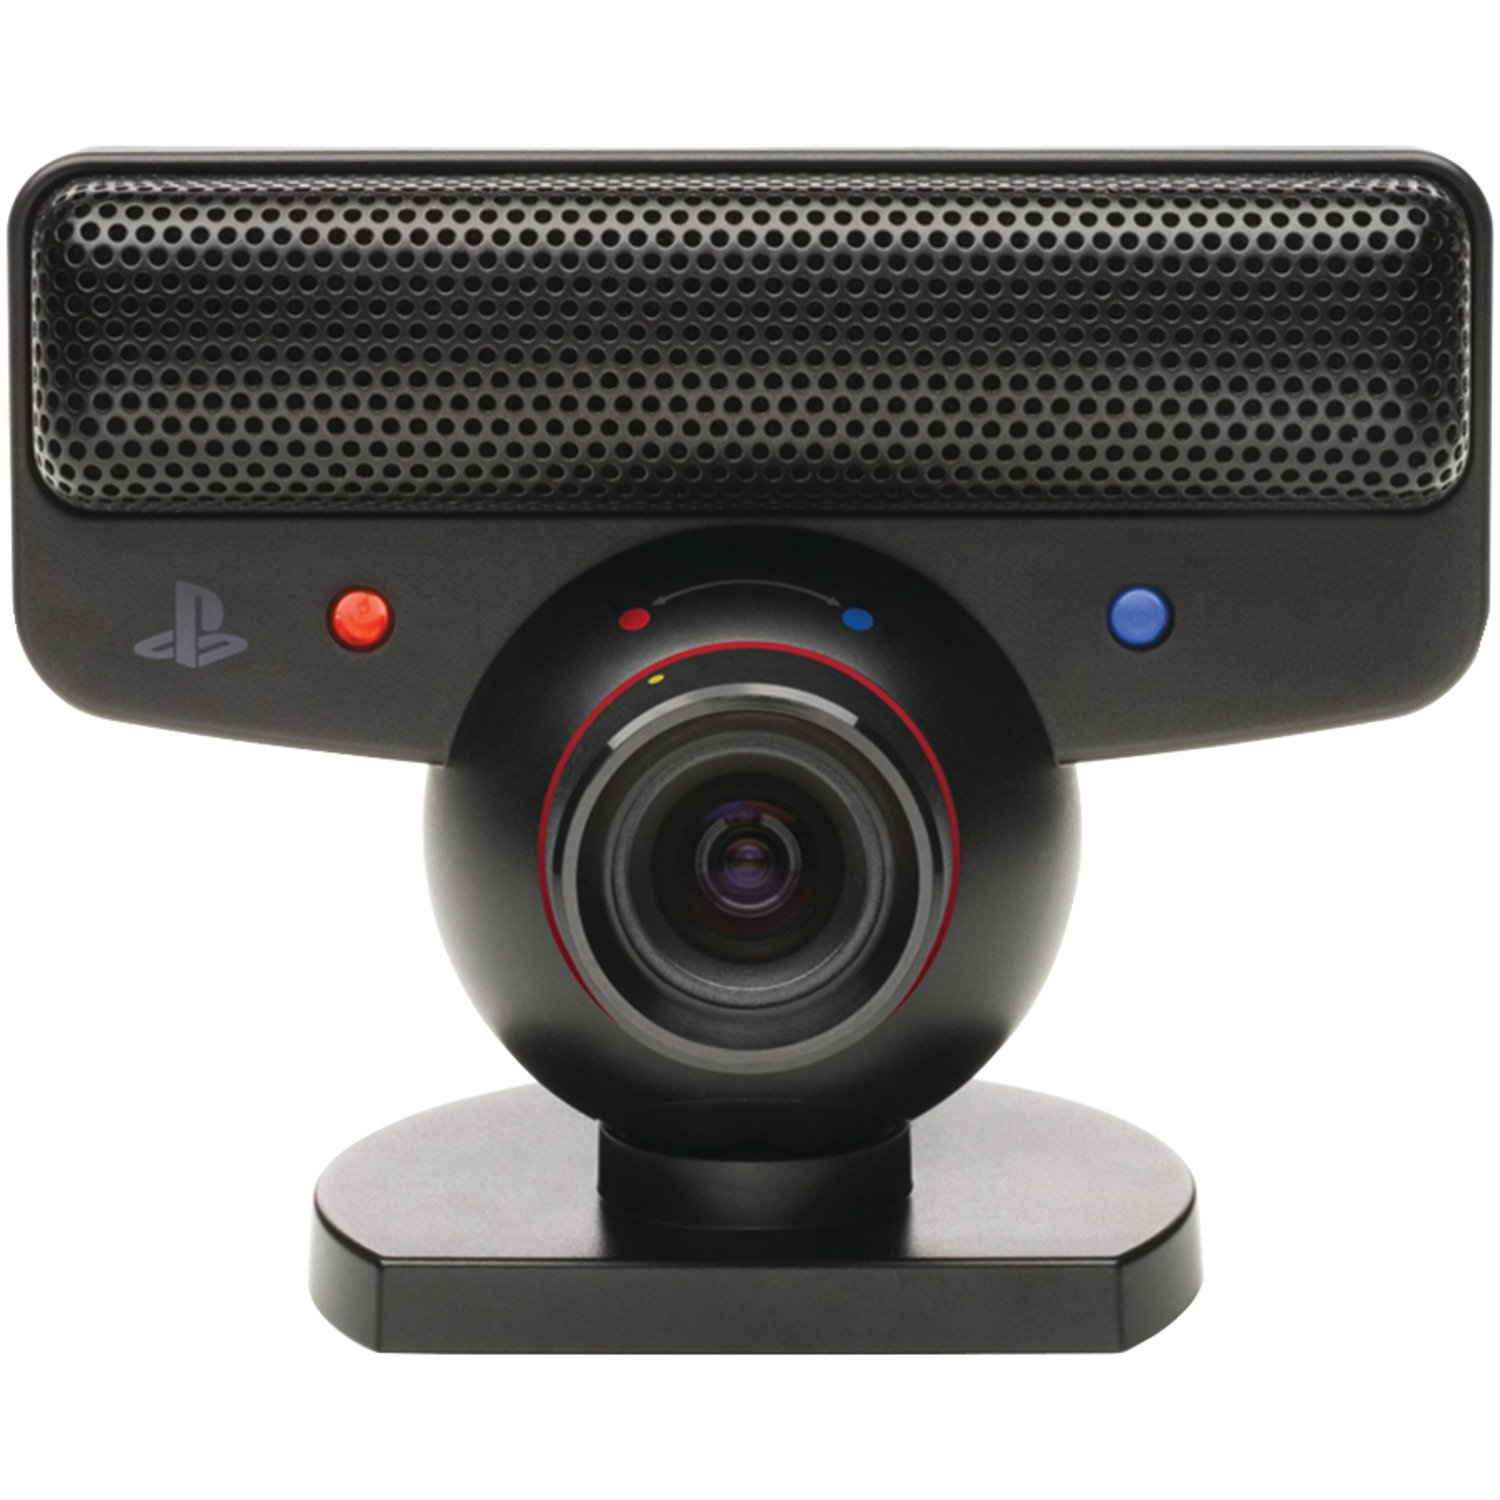
\includegraphics[width=0.3\textwidth]{./Imagenes/Bitmap/PSEye.jpg}
     }
     \caption{Dispositivos de entrada relevantes de Xbox y PlayStation en la 7"a  generaci\'on}
     \label{fig:septima2}
   \end{figure}

En 2010 Microsoft dio el salto a un nuevo controlador de videojuegos para su consola Xbox 360. Este nuevo perif\'erico es conocido con el nombre de \textbf{Kinect} (figura~\ref{septa3}) y permite a los usuarios controlar e interactuar con la consola sin necesidad de tener contacto f\'isico con un mando tradicional. Este control se realiza por gestos y reconocimiento de voz. El sensor Kinect es una barra horizontal de unas 9 pulgadas conectada a una peque\~na base circular con un eje que permite que esta rote. Adem\'as est\'a dise\~nado para ser colocado por encima o por debajo de la televisi\'on. El dispositivo cuenta con una c\'amara RGB, un sensor de profundidad, un micr\'ofono de m\'ultiples matrices y un procesador personalizado que ejecuta el software patentado, que proporciona captura de movimiento de todo el cuerpo en 3D, reconocimiento facial y capacidades de reconocimiento de voz. El micr\'ofono de matrices del sensor de Kinect permite a la Xbox 360 llevar a cabo la localizaci\'on de la fuente ac\'ustica y la supresi\'on del ruido ambiente, permitiendo participar en el chat de Xbox Live sin utilizar auriculares. El sensor de profundidad es un proyector de infrarrojos combinado con un sensor CMOS monocromo que permite a Kinect ver la habitaci\'on en 3D en cualquier condici\'on de luz ambiental. El rango de detecci\'on de la profundidad del sensor es ajustable gracias al software de Kinect capaz de calibrar autom\'aticamente el sensor, basado en la jugabilidad y en el ambiente f\'isico del jugador, tal como la presencia de sof\'as, mesas y otro tipo de muebles.\\

PlayStation tambi\'en lanz\'o al mercado su sistema de control de videojuegos por movimiento, \textbf{PlayStation Move} (figura~\ref{septa4}), y es compatible con los sitemas PS3 y PS4. PlayStation Move compiti\'o tanto con el Kinect de Xbox como con el WiiMote de Nintendo. Para poder utilizar PlayStation Move se necesitan 3 componentes: \textit{Motion Controller, Navigation Controller y PlayStation Eye} (figuras~\ref{septa4} y \ref{septa5}). Motion Controller es el mando principal y tiene una forma alarga con una esfera luminosa en su parte superior. Esta esfera es utilizada para que PlayStation Eye detecte el mando. Esta c\'amara lee los movimientos del mando para posteriormente ser interpretados por el juego. Como complemento al Motion Controller, existe el Navigation Controller. Este controlador cumple la misma funci\'on que el Nunchuck de Wii. \\

%%%%%%%%%%%%%%%%%%%%%%%%%%%%%%%%%%%%%%%%%%%%%%%%%%%%%%%%%%%%%%%%%%

\subsection{Octava generaci\'on (2012-2020)}

Coincidiendo con la salida al mercado del PlayStation Move, Nintendo lanz\'o su nueva consola en 2012; la \textbf{Wii U} y con ella un controlador de videojuegos h\'ibrido. Este controlador h\'ibrido es el \textbf{Wii U GamePad} y es el mando principal de la consola. La principal distinci\'on con respecto a los mandos tradicionales es la incorporaci\'on de una pantalla t\'actil (figura~\ref{octava1}), la cual se utiliza para mostrar informaci\'on adicional durante una partida y adem\'as puede usarse como pantalla principal en caso de no disponer de un televisor mientras se juega. Adem\'as de como controlador de videojuegos, el Wii U GamePad es utilizado como control remoto independiente para cotrolar la pantalla de la televisi\'on u otro aparato via infrarrojos sin necesidad de tener la consola encendida. El mando contaba con altavoces y micr\'ofono e incorporaba una c\'amara frontal de 1.3 megapixeles. Los sensores que incorporaba eran: aceler\'ometro, giroscopio, geomagn\'etico e infrarrojo e incorporaba vibraci\'on. La conexi\'on a la consola se hac\'ia mediante bluetooth  y dispon\'ia de NFC para futuros accesorios que incorporaron a los diferentes videojuegos.\\

\begin{figure}[t]
     \subfloat[Wii U Gamepad\label{octava1}]{%
       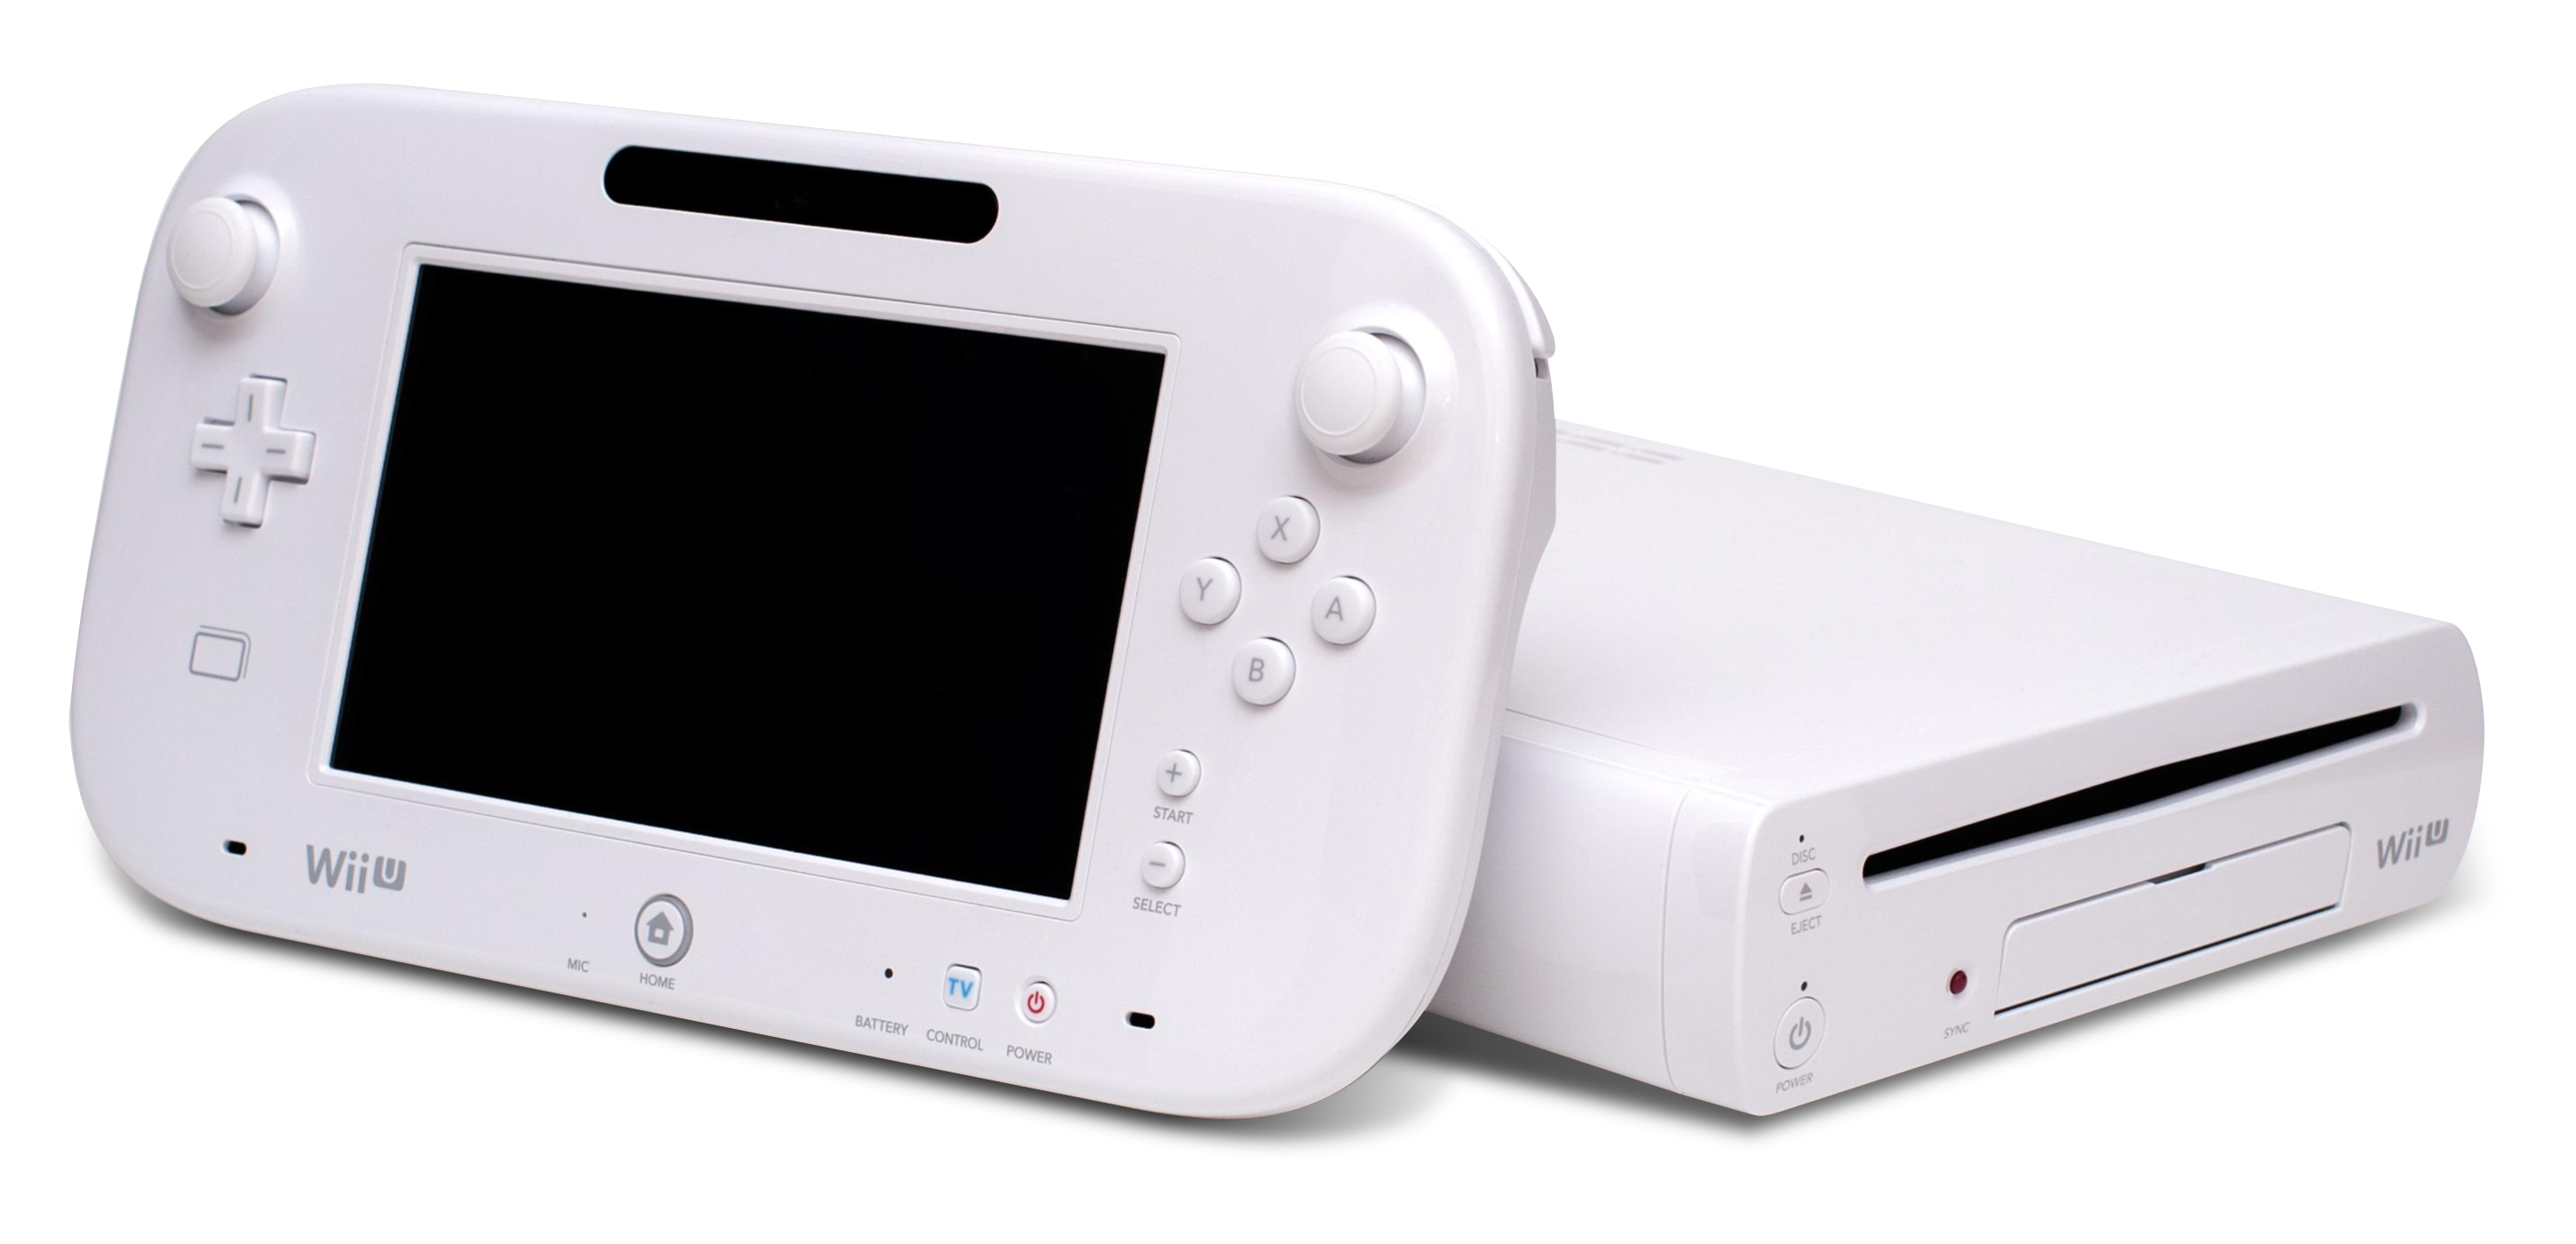
\includegraphics[width=0.3\textwidth]{./Imagenes/Bitmap/Wii_U_Console_and_Gamepad.png}
     }
     \hfill
\subfloat[Dualshock 4\label{octava2}]{%
       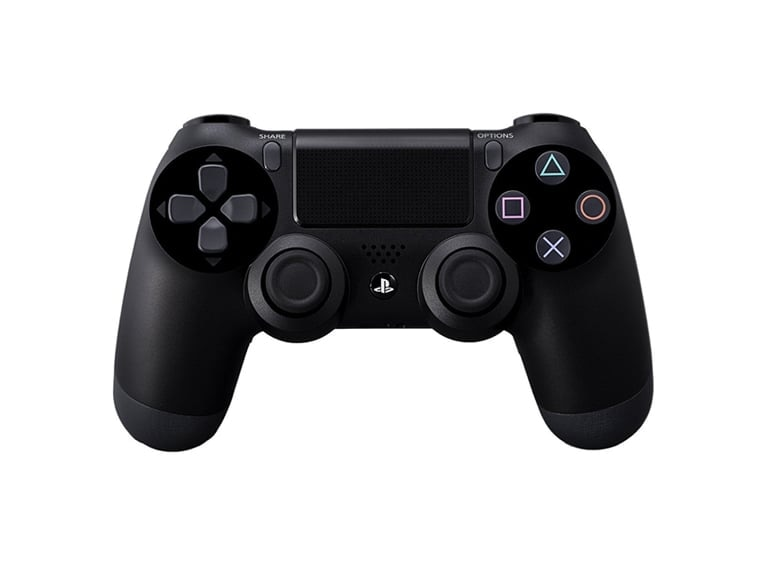
\includegraphics[width=0.3\textwidth]{./Imagenes/Bitmap/Dualshock4.jpg}
     }
\hfill
\subfloat[Xbox One Elite Controller\label{opctava3}]{%
       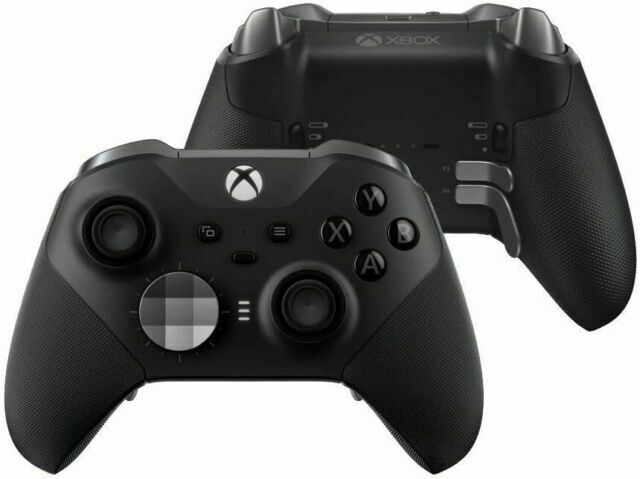
\includegraphics[width=0.3\textwidth]{./Imagenes/Bitmap/Xbox One Elite Controller.jpg}
     }
     \caption{Dispositivos de entrada relevantes en la 8"a  generaci\'on}
     \label{fig:octava}
   \end{figure}

En 2013 Sony hizo una revisi\'on de su DualShock y como mando de la consola PlayStation 4 lanz\'o el \textbf{DualShock 4} (figura~\ref{octava2}). Este mando a\~nadi\'o al dise\~no anterior un panel t\'actil en la parte frontal, lo que hizo que la distribuci\'on de los botones que antes eran centrales cambiasen. En la parte trasera se a\~nadi\'o una barra LED que se ilumina en varios colores para diferenciar e identificar a los diferentes jugadores. Microsoft por su parte en 2015 puso a la venta su nuevo \textbf{Xbox One Elite Controller}. Una de las principales caracter\'isticas es que tiene un dise\~no modular por lo que cada pieza es intercambiable para que cada jugador pueda adaptarlo a su medida. La personalizaci\'on es el principal aliciente en este mando ya que permite reprogramar tanto los cuatro botones tradicionales de la parte frontal como los gatillos. Tambi\'en se da la posibilidad de establecer curvas de sensibilidad en las palancas anal\'ogicas. Gracias a la posibilidad de a\~nadir piezas, este mando incluye 4 palancas m\'as en la parte trasera como puede verse en la figura~ \ref{octava3}.\\

\begin{figure}[t]
     \subfloat[Par de Joy-Cons desacoplados\label{octava4}]{%
       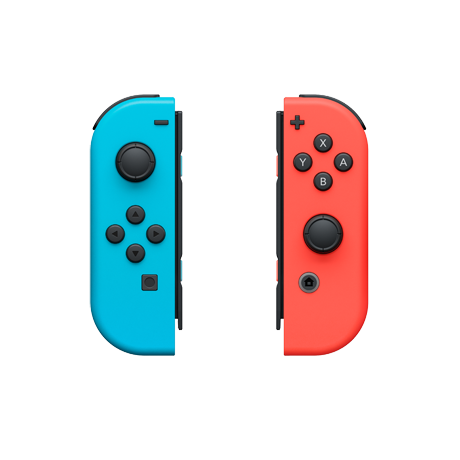
\includegraphics[width=0.5\textwidth]{./Imagenes/Bitmap/Joy-Con.png}
     }
     \hfill
\subfloat[Nintendo Switch\label{octava5}]{%
       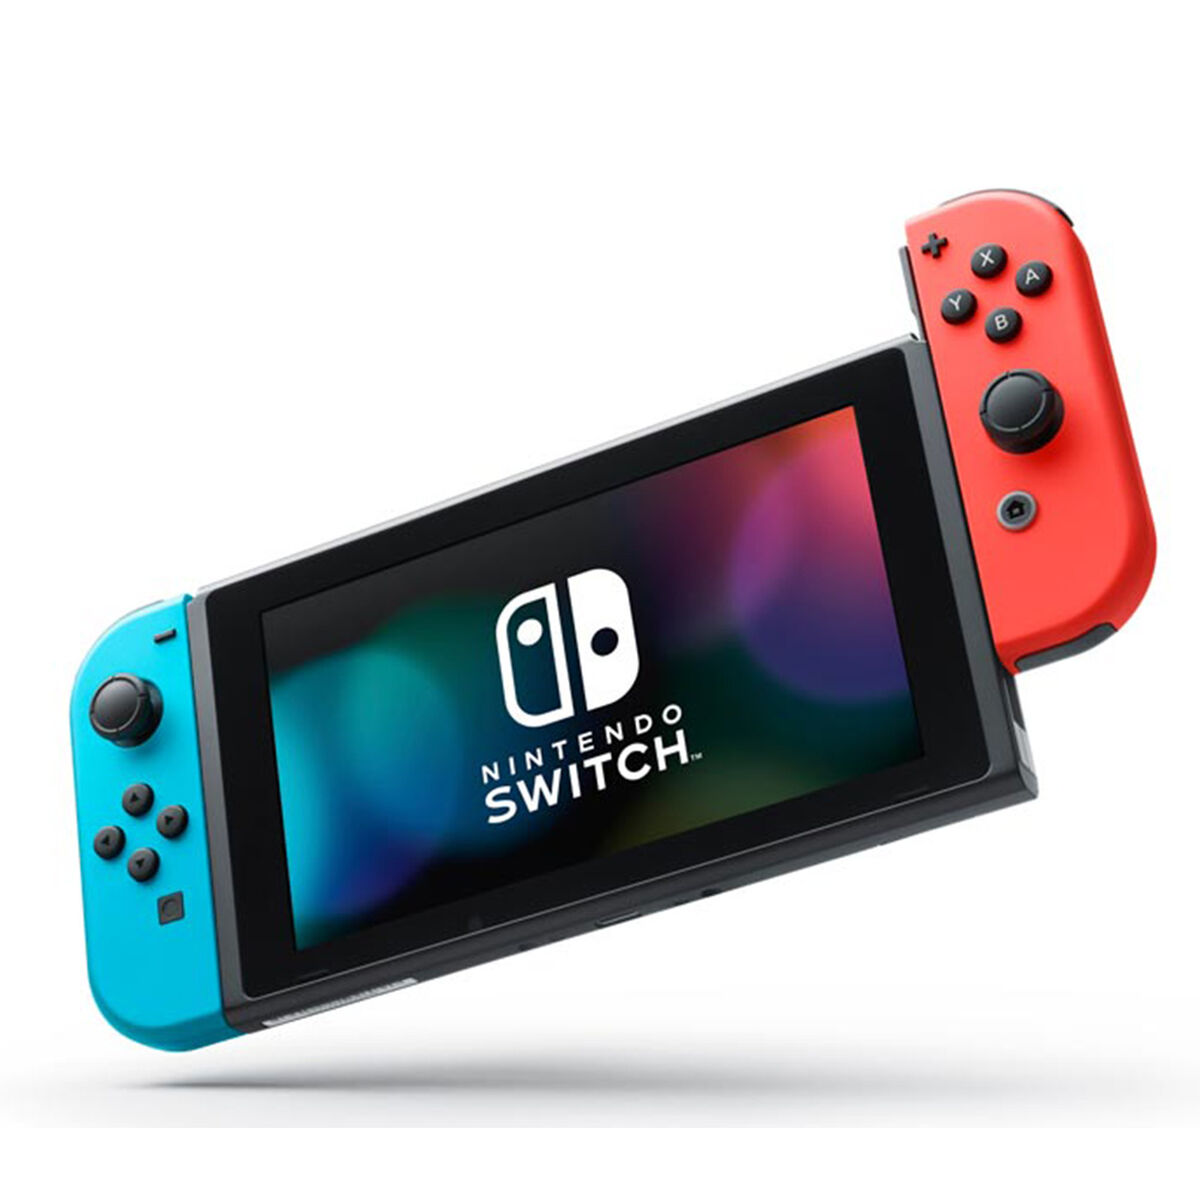
\includegraphics[width=0.4\textwidth]{./Imagenes/Bitmap/switch.jpg}
     }
     \caption{Nintendo Switch}
     \label{fig:octava2}
   \end{figure}

En 2017 Nintendo present\'o su nueva consola h\'ibrida que que tiene como base Wii U. La consola es \textbf{Nintendo Switch} (figura~\ref{octava5}) y es una consola que puede ser jugada tanto de manera port\'atil como en formato sobremesa con una televisi\'on o un monitor. Los mando dise\~nados para esta consola son los \textbf{Joy Con} y consisten en 2 unidades, cada uno de ellos contiene una palanca anal\'ogica y una matriz de botones. Estos mandos tienen la peculiaridad de que pueden usarse tanto acoplados a la consola o por separado. Cada uno de los Joy-Con puede ser utilizado como mando individual y se distribuyen en pares, designados como Joy-Con L y Joy-Con R. Una misma Nintendo Switch puede tener conectados hasta un total de 8 Joy-Con para juegos multijugador.\\

La comunicaci\'on que tienen los mandos con la consola se realiza por bluetooth gracias a una bateria no extraible de 525 mAh en cada mando. Ambos controladores contienen una palanca anal\'ogica, cuatro botones en su parte frontal, dos botones superiores, dos botones laterales accesibles cuando se desacoplan de la consola, un bot\'on - para el Joy-Con L y un bot\'on + para el Joy-Con R y un indicador de jugador luces LED (figura~\ref{octava4}). Cada uno de los Joy-Con contiene un aceler\'ometro y un giroscopio, que pueden ser utilizados para los juegos que incluyen movimiento. Adem\'as, el Joy-Con R contiene un sensor de seguimiento de profundidad infrarroja, que puede leer objetos y movimientos sostenidos delante de \'el. Cada uno de los Joy-Con incorpora un motor para hacer vibrar el mando durante las sesiones de juego.\\

Tambi\'en durante 2017, Sony anunci\'o una serie de juegos nuevos que se jugar\'ian de una forma totalmente diferente ya que el mando utilizado ser\'ia cada uno de los tel\'efonos m\'oviles de los usuarios. A esta serie de juegos se la conoce como \textbf{PlayLink}. La idea detr\'as de PlayLink es que todos los usuarios de la consola PlayStation 4 y sus familiares y amigos disponen de un dispositivo m\'ovil pero no todos disponen de varios mandos para poder jugar con m\'as personas en juegos cooperativos. PlayLink es una aplicaci\'on m\'ovil que cada usuario se descarga en su Android o iOS y as\'i puede usar su tel\'efono como un mando m\'as de PlayStation 4. El requisito para que la conexi\'on sea efectiva es que tanto la consola PS4 como los dispositivos m\'oviles que se vayan a usar est\'en conectados a la misma red WIFI.\\

%%%%%%%%%%%%%%%%%%%%%%%%%%%%%%%%%%%%%%%%%%%%%%%%%%%%%%%%%%%%%%%%%%

\subsection{Novena generaci\'on (2020-Actual)}

\begin{figure}[t]
\centering
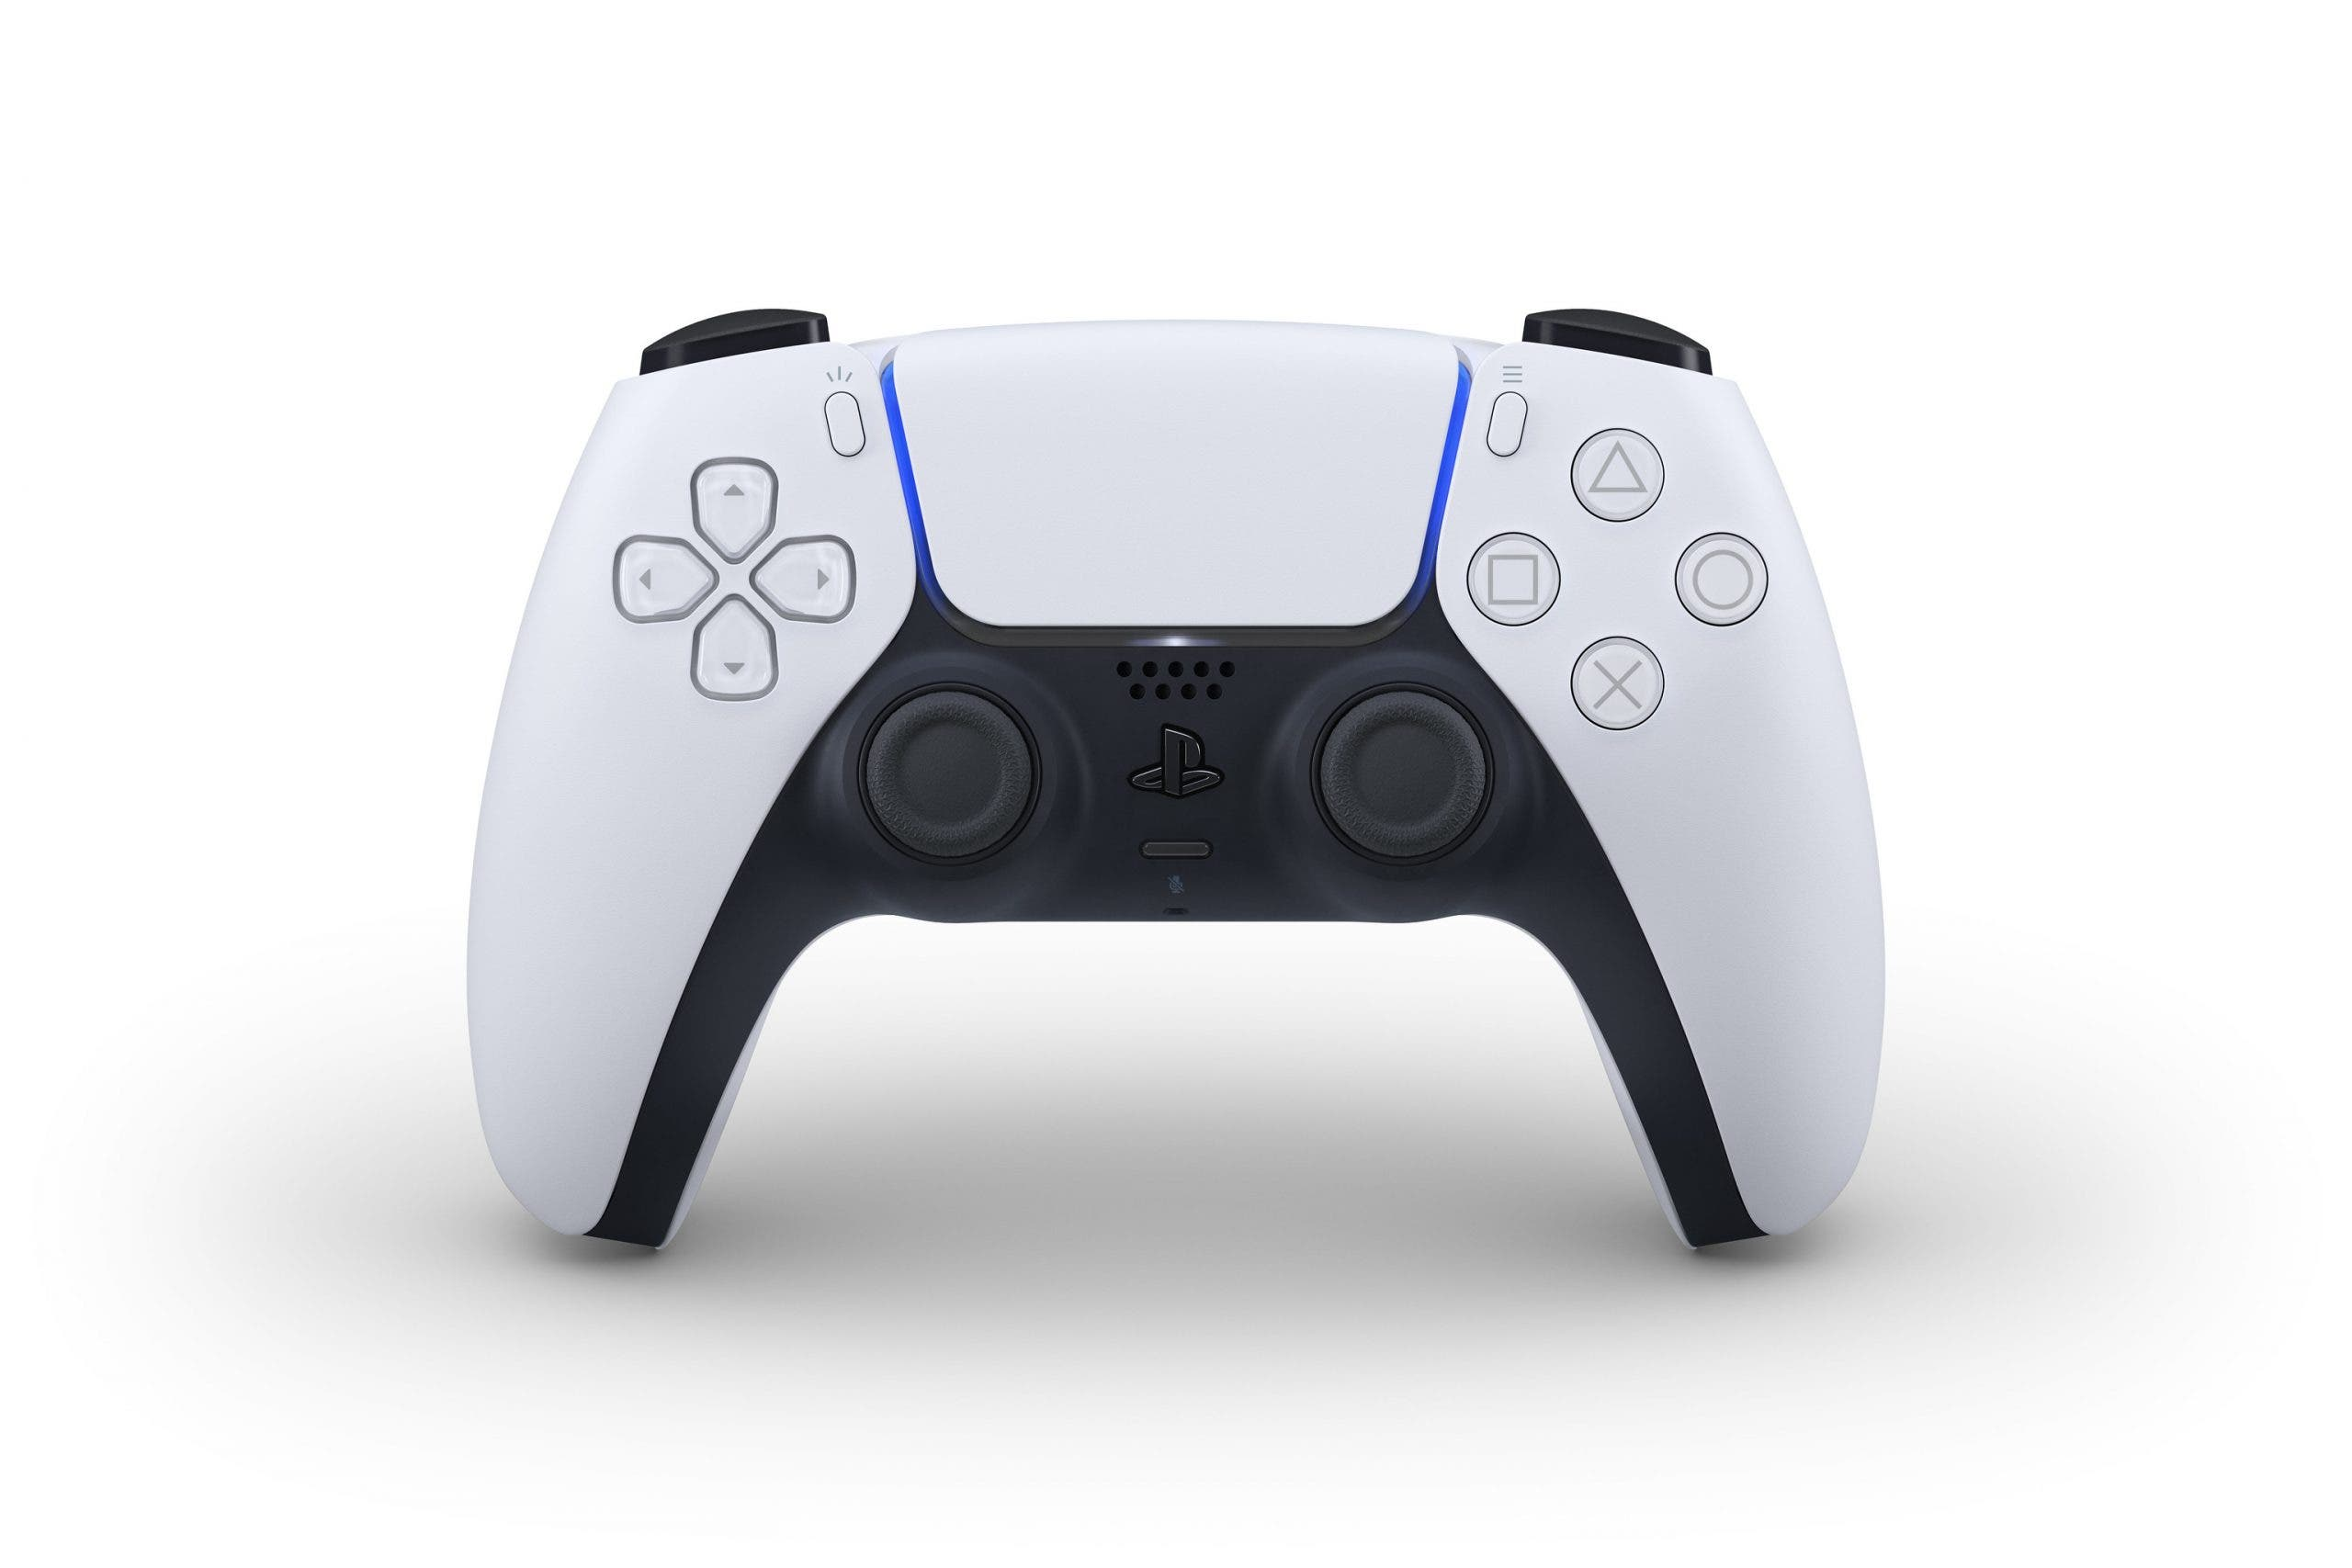
\includegraphics[width=0.4\textwidth]{./Imagenes/Bitmap/dualsense.jpg}
\caption{PS5 Dualsense Controller}
\label{Fig:dualsense}
\end{figure}

A finales del a\~no 2020 Sony lanz\'o al mercado su nueva consola, la PS5 y con ella un nuevo mando al que bautizaron como \textbf{DualSense} (figura~\ref{Fig:dualsense}). Como ya pasaba con el DualShock 4, este mando funciona con bater\'ia y lleva un altavoz integrado. La gran novedad que trae este mando es la retroalimentaci\'on h\'aptica. Se han sustituido los motores de vibraci\'on tradicionales por 2 activadores que emiten vibraciones din\'amicas capaces de simular todo tipo de sensaciones. Adem\'as de la nueva retroalimentaci\'on h\'aptica, el nuevo DualSense incorpora 2 gatillos adaptativos. Estos gatillos emiten diferente fuerza de resistencia contra el jugador dependiendo del arma que se est\'e utilizando. El ejemplo que pusieron los desarrolladores de Sony fue con la cuerda de un arco, inicialmente no tiene resistencia pero cuanto m\'as se tense la cuerda del arco m\'as fuerza es necesaria.

\section{\textit{Feedback} en los controladores}

En los inicios de los videojuegos y de las consolas el objetivo fue la creaci\'on de nuevos tipos de juegos con diferentes mec\'anicas y mejoras gr\'aficas. En la era actual de los videojuegos se ha ido mucho m\'as lejos de los primeros juegos como Pong y Tetris, la tendencia ha llevado a la creaci\'on de escenarios virtuales m\'as realistas y a que el jugador formase parte de ese entorno virtual. Particularmente la respuesta que se da al usuario del videojuego al realizar acciones es conocida como \textbf{tecnolog\'ia h\'aptica}. Este tipo de tecnolog\'ia se refiere al conjunto de interfaces tecnol\'ogicos que interaccionan con una persona mediante el sentido del tacto. La tecnolog\'ia h\'aptica tiene sus inicios en los dispositivos de los sistemas servo para controlar grandes aviones con la intenci\'on de poder hacerlo de manera remota. En estos sistemas se instal\'o un sistema de control que proporcionaba una resistencia a la palanca del piloto proporcional al \'angulo de ataque del avi\'on. Otro ejemplo destacable de esta tecnolog\'ia se encuentra en la pel\'icula \textbf{4-D Honey, I Shrunk the Audience!} del a\~no 1994 que simulaba que los ratones se soltaban por el auditorio y corrian por toda la sala. Para conseguir esta simulaci\'on se bombeaba aire a trav\'es de un peque\~no tubo de pl\'astico y al agitarse, imitaba la sensaci\'on de las colas de los ratones rozando las piernas de los espectadores. \\

En los videojuegos esta tecnolog\'ia fue introducida a trav\'es de los controladores. Al inicio estos sistemas de vibraci\'on se introdujeron en los controladores como dispositivos que se acoplaban al mando por separado como pasaba con el \textbf{Rumble Pack} de Nintendo 64. Con la salida del \textbf{Dualshock} en su versi\'on japonesa esto cambi\'o. Este mando incorporaba un sistema de vibraci\'on conocido como \textit{tabletas vibradoras (rumble packs)} que ten\'ian ese efecto de vibraci\'on al conducir veh\'iculos o disparar armas de fuego. Con la llegada de las pantallas t\'actiles tambi\'en aparecieron las pantallas h\'apticas. Estas pantallas son aquellas que transmiten una vibraci\'on al tocarla. El ejemplo m\'as actual de tecnolog\'ia h\'aptica puede encontrarse en la reciente consola de Nintendo, Nintendo Switch. Nintendo no ha denominado a la tecnolog\'ia que usan sus Joy-Cons como tecnolog\'ia h\'aptica sino como \textbf{Rumble HD}. \\

\begin{figure}[t]
     \subfloat[Force Feedback Pro\label{feedback1}]{%
       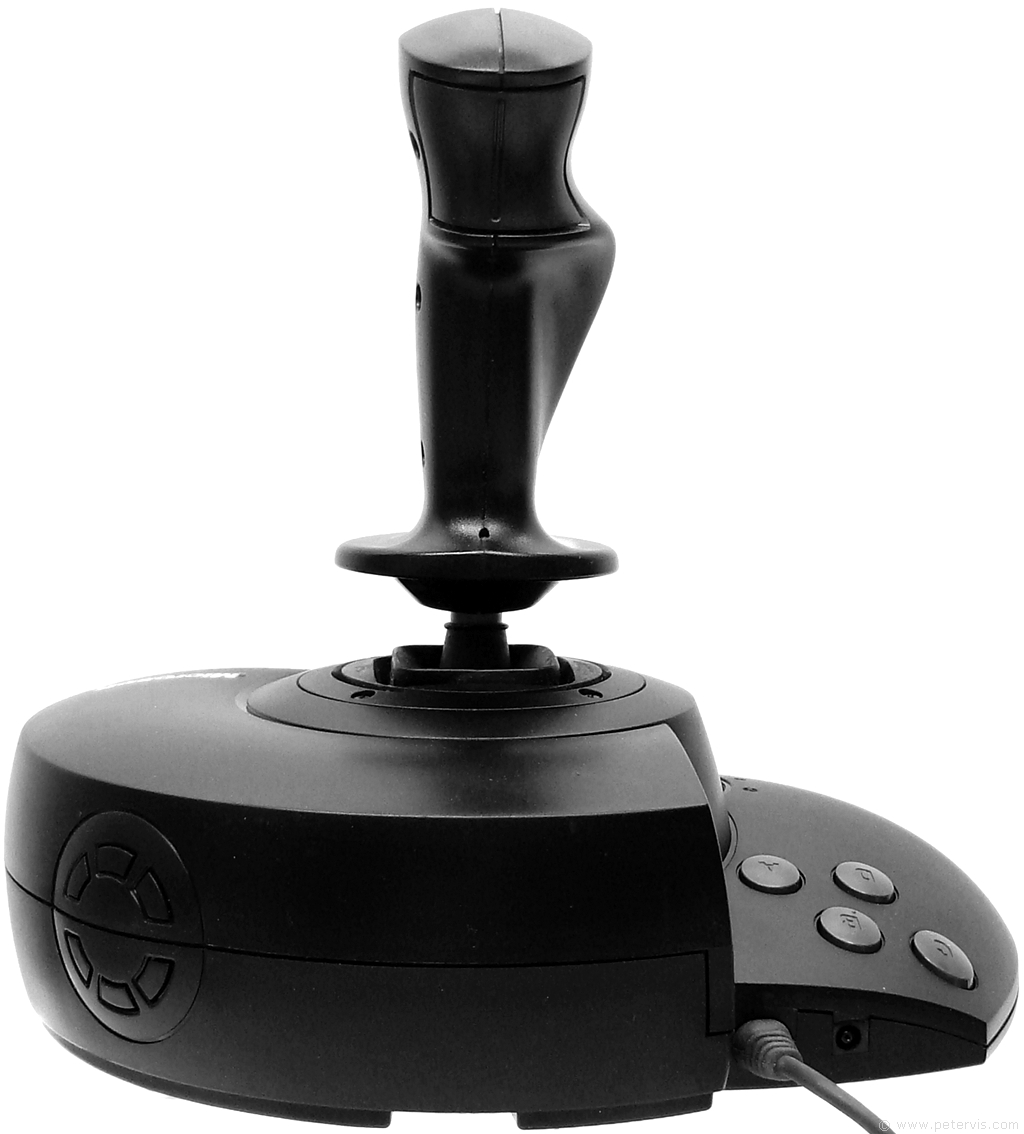
\includegraphics[width=0.4\textwidth]{./Imagenes/Bitmap/sidewinder-force-feedback-pro-back-view.jpg}
     }
     \hfill
\subfloat[Microsoft Sidewinder Force Feedback Wheel\label{feedback2}]{%
       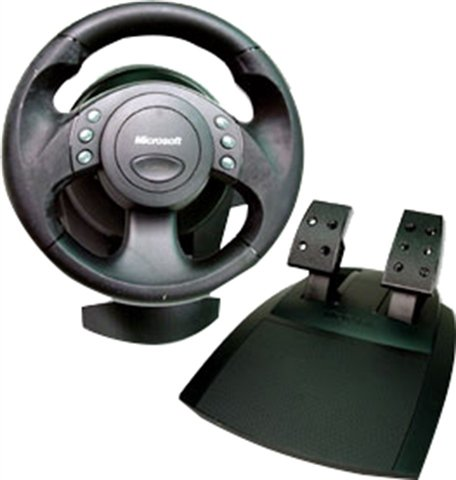
\includegraphics[width=0.4\textwidth]{./Imagenes/Bitmap/SACCMICFFW_l.jpg}
     }
     \caption{Primeros dispositivos con \textit{force feedback}}
     \label{fig:feedback}
   \end{figure}

El mundo de la simulaci\'on trata de intentar recrear el mundo real dentro de un videojuego. En este tipo de juegos de simulaci\'on la respuesta que recibe el usuario importa mucho debido al caracter inmersivo que puede llegar a ofrecer. Para lograr esto, en 1997 Microsoft sac\'o al mercado un producto que inclu\'ia \textit{force feedback}, Force Feedback Pro (figura~\ref{feedback1}). Como este dispositivo estaba pensado para su uso en PC, los puertos eran \'unicamente de entrada. Para conseguir enviar datos desde el ordenador al dispositivos era necesario utilizar las capacidades que dispon\'ia este puerto para poder usar MIDI. Esto quiere decir que los primeros mensajes de vibraci\'on ven\'ian dados por mensajes MIDI y que ordenadores que no tuvieran la posibilidad de usar este puerto, no podr\'ian utilizar la funci\'on de vibraci\'on de los mandos. En ese mismo a\~no, Microsoft sac\'o al mercado el que ser\'ia el primer volante con retroalimentaci\'on (figura~\ref{feedback2}). Este ser\'ia el primer volante para jugar fuera de las m\'aquinas recreativas arcade.\\



\section{Sistemas de \textit{streaming} en videojuegos}

Con la extensi\'on de los dispositivos m\'oviles en el mundo de los videojuegos y las mejoras en las conexiones a internet, la industria de los videojuegos se mueve a pasos acelerados hacia el \textit{gaming} en la nube. Servicios de retransmisi\'on via streaming como \textit{Netflix} o \textit{Amazon Prime Video} ofrecen la posibilidad de disponer de un cat\'alogo de series a peliculas a trav\'es de internet. Con este precedente, empresas como Google\footnote{https://stadia.google.com/} y Nvidia\footnote{https://www.nvidia.com/es-es/geforce-now/} se han adentrado al mundo de los juegos en la nube.\\

Esta nueva forma de forma no solamente consiste en retransmitir al usuario final ala partida que est\'a jugando sino que el proceso va mucho m\'as all\'a. Esta diferencia tiene lugar a la hora de tratar el input del usuario. En un videojuego tradicional, ejecutado en la misma m\'aquina en la que se est\'a jugando, una vez el usuario realiza una entrada el videojuego lo procesa y genera una respuesta apropiada. En los videojuegos en la nube una vez el usario realiza una acci\'on, esta debe ser enviada al servidor donde el juego est\'a siendo ejecutado. Una vez en el servidor, la entrada que gener\'o el usuario es tratada y se realizan los cambios en el estado del juego que haya probocado el usuario con su entrada. Cuando el estado cambia en el servidor se prepara el frame, se codifica y es enviado de vuelta al usuario que tendr\'a que decodificar el frame una vez le llegue al dispositivo donde est\'e jugando \citep{cloudgaming}.

Los anchos de banda requeridos para estas dos tecnolog\'ias var\'ian con las resoluciones a las que se quiera jugar (tabla~\ref{stadiovsgeforce}). Ambos sistemas aconsejan una conexi\'on Ethernet o un router que disponga de una red de frecuencia 5 GHz.

\begin{table}[h]
    \begin{tabular}{lll}
        \toprule
         & \textbf{Google Stadia} & \textbf{Nvidia GeForce Now} \\
        \midrule
        \textbf{720p 60fps} & 10 Mbps & 15 Mbps\\
        \textbf{1080p 60fps} & 20 Mbps & 25 Mbps \\
		\textbf{4K 60fps} & 35Mbps & No Disponible \\
        \bottomrule
    \end{tabular}
\caption{Ancho de banda necesario para jugar a Stadia vs GeForce Now}
\label{stadiovsgeforce}
\end{table}


En los sistemas de streaming de video convencionales se utiliza la t\'ecnica conocida como \textit{buffering}. Esta t\'ecnica puede realizarse siempre y cuando la conexi\'on a internet sea lo suficientemente r\'apida como para descargar un fragmento de los datos que van a usarse a continuaci\'on antes de necesitarlos. Con esto lo que se consigue es aprovechar los momentos en los que se dispone de un ancho de banda mayor para descargar parte del contenido que se va a visualizar a continuaci\'on. Esto permite al usuario no ser consciente de retrasos moment\'aneos en la red. En el mundo de los juegos en la nube este proceso se ve truncado por la interacci\'on del usuario. El juego no puede predecir lo que va a pasar por lo que no se puede hacer \textit{buffering} de los frames. Este hecho convierte a los sistemas de juegos en la nube en sistemas sensibles a los retrasos en la red.\\

\begin{figure}[h]

\centering
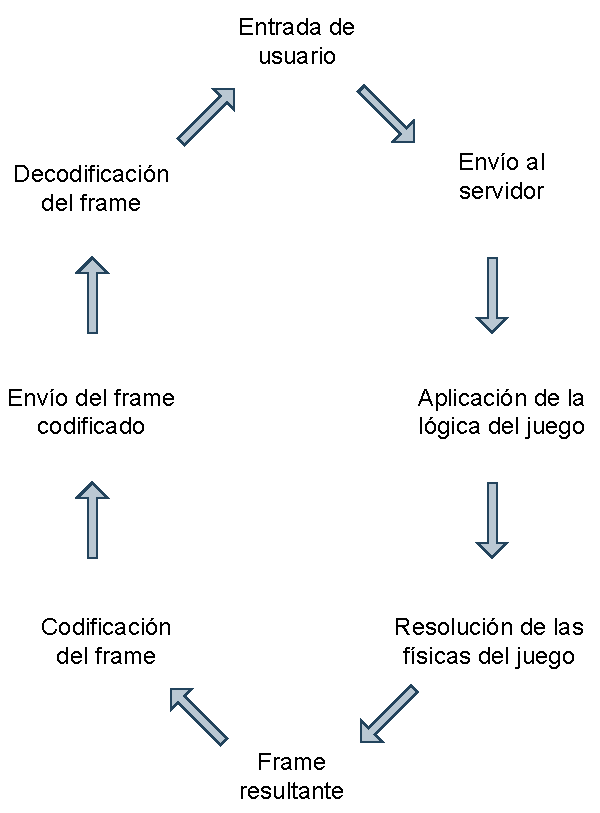
\includegraphics[width=0.6\textwidth]{./Imagenes/Vectorial/cloudgaming cycle.pdf}
\caption{Flujo de la entrada de usuario de juegos en la nube}
\label{cycle}
\end{figure}

En los juegos que se transmiten por red, una vez el usuario ha realizado la pulsaci\'on, esta pulsaci\'on es transmitida al servidor de manera encriptada. Una vez la entrada del usuario llega al servidor, debe ser desencriptada y los cambios deben aplicarse en el juego. Una vez aplicados los cambios, el frame debe ser codificado y transmitido de vuelta al usuario. El usuario decodifica el frame y lo muestra. Este ciclo se repite constantemente en el ciclo de los juegos en la nube (ver figura~\ref{cycle}).\\

El inter\'es de los jugadores por un producto depende de muchos aspectos. Uno de los principales es la experiencia que el usuario recibe al jugar. Esto hace que una caida del servicio mientras el jugador est\'a jugando puede crear una frustraci\'on en el usuario y hacer que este pierda el inter\'es. La latencia est\'a definida como el tiempo de respuesta entre el servidor donde se est\'a ejecutando el juego y el cliente que est\'a jugando. Existen diferentes tipos de latencias o retrasos en la red. El m\'as com\'un es el retraso en la renderizaci\'on del siguiente frame. \\

En este proyecto todos estos inconvenientes convergen. El uso de la red requiere de un m\'inimo ancho de banda y es por esto que tal y como se hablaba al principio del cap\'itulo, los sistemas como Stadia piden unas m\'inimas velocidades para poder asegurar la fluidez a la hora de jugar. Un juego que ejecute a 60 frames por segundo quiere decir que se disponen de 16 segundos aproxim\'adamente para realizar el ciclo comentado en la figura~\ref{cycle}. En ocasiones para conseguir mantener estas tasas de frames se realiza una disminuci\'on de la calidad gr\'afica con la que llega el frame. Realizar estos cambios din\'amicos de manera puntual en picos donde el uso del ancho de banda es demasiado ayuda a que el jugador no tenga desconexiones o retrasos en la entrada que ha realizado.\\


%-------------------------------------------------------------------


% Variable local para emacs, para  que encuentre el fichero maestro de
% compilaci�n y funcionen mejor algunas teclas r�pidas de AucTeX
%%%
%%% Local Variables:
%%% mode: latex
%%% TeX-master: "../ManualTeXiS.tex"
%%% End:
